\chapter{Group theory and representation of the Lorentz group}
\section{Group Theory}
\subsection{Introduction}
Symmetries in physics will be related to groups and will constrain the possible terms in the Lagrangian. This means that the theory can be solved exactly in particular cases, this property is called \emph{integrability}.\\
The following continuous symmetries are realized in nature:
\begin{enumerate}
	\item Rotational symmetry $SO(3)$ (i.e. rotate lab or experiment, invariant)
	\item Lorentz symmetry $S0(3,1)$ (experiment in inertial system same as in laboratory system)
	\item Gauge, Flavour symmetry e.g. $SU(3)$ (scattering experiments are invariants)
\end{enumerate}
Continuous symmetries are represented by Lie groups. Discrete symmetries on the other hand are
\begin{enumerate}
	\item Parity $\vec{x}\rightarrow-\vec{x}$
	\item charge conjugation $e^- \rightarrow e^+$
	\item time reversal $t \rightarrow-t$
\end{enumerate}
Note that the CPT symmetry always holds for the weak force, compare \ref{eq:cpttheorem}. CP symmetry holds valid for EM and QCD.
\subsection{Lie-Group, Lie-Algebras and their Representations}
A Lie group is a group which is also a differentiable manifold, a group whose elements can be labelled at least locally by a set of continuous variables. Everything (multiplication, inverse, representation etc) should depend smoothly on these parameters. The dimension of a Lie group is given by the number of these parameters.
\marginpar{$O(n),U(n)$} 
\begin{mybox}{Lie group} 
	A \emph{Lie-group} is a group with the structure of a smooth manifold, ie.e. its differentiable (in the sense that it is equipped with a differentiable map) structure is compatible with the group. Lie groups are therefore groups which are also manifolds, such that the group action is a diffeomorphism. \\
\end{mybox}
The map goes from parameter space in $\mR^n$ to the manifold and thus assigns an element of parameter space to an element of the group, i.e. the manifold. The group action $g_{\alpha_1} g_{\alpha_2} =g_{\alpha_3}, g_{\alpha} \in G$, induces a link between elements of parameter space. The map satisfies the group laws.\\

\subsubsection{Lie algebras}
The Lie algebra generates (i.e. it is not part of the Lie group) elements of the Lie group infinitesimally close to the identity.
\begin{mybox}{Lie-algebra}
	A Lie-algebra $\mathcal{g}=$Lie$G$ is a vector space with a bilinear antisymmetric operation
	\begin{equation}
	\circ: \mg \times \mg \rightarrow \mg, \quad (a,b) \mapsto [a,b]
	\end{equation}
	with the properties
	\begin{align}
		i) \quad A\circ B &= - B\circ A \quad \Rightarrow 0 = [,]\\
		ii)\quad A\circ(B\circ C) &+ B\circ (C\circ A) + C\circ (A\circ B) = 0.
	\end{align}
	A Lie-algebra of finite dimension is defined by $[,]=0$ on the basis of the vector space, i.e. with
	\begin{equation}
	x_A \circ x_B = f^C_{\, AB} x_C,
	\end{equation}
	where $f^C_{\,AB}$ are called \emph{structure constants} of the Lie algebra. They have the properties:
	\begin{align}
		i) \quad f^C_{\, AB} &= - f^C_{\, BA} \\
		ii) \quad f^D_{\, AB} f^E_{\, CD} &+ f^D_{\, CA} f^E_{\, BD} + f^D_{\, BC} f^E_{\, AD} =0.
	\end{align}
	In general, a basis $T^A$ of a Lie algebra satisfies
	\begin{equation}
	[T^A,T^B]= \sum_C i f^{AB}_{\,\, C} T^C.
	\end{equation}
\end{mybox}
\subsubsection{Example on how to count these parameters}
Consider $SO(3)$, it describes rotations around a given axis in $\mR^3$, hence in the $(x,y),(y,z),(x,z)$ plane. These rotations can be generated by the basis elements, i.e. the generators, of the associated Lie group $so(3)$. This basis is the basis for a $3d$ vector space of antisymmetric $3\times3$ matrices. We make an ansatz for the elements of $SO(3)$:
\begin{equation}
	A = \mathcal{I}+\epsilon a + \mathcal{O}(\epsilon^2)
\end{equation}
such that we find
\begin{equation*}
	A^T A = \mI = \mI + \epsilon (a + a^T) + \mathcal{O}(\epsilon^2) \; \Leftrightarrow\; a^T=-a
\end{equation*}
such that the antisymmetric matrices form the basis for the vector space, as we stated above\\
We do not in general get all elements of the Lie group by means of generating them with an exponential map, as we can only map to those elements which are connected to the identity, i.e. the exponential map is not bijective.\\
However, it should normally suffice, but for the spinor representation of $SU(2)$ we only get a pseudo representation of $SO(3)$ by means of the exponential map, since $SU(2)$ is the double cover of $SO(3)$, cf. below.\\
Now onto counting:
\begin{mybox}{}
	The dimension of a Lie algebra as a vector space is the dimension of the Lie group, which then again is equal to the number of parameters.
\end{mybox}
Therefore, we can find the dimension of the Lie group, i.e. the number of parameters by e.g. counting the number of basis elements of the associated Lie algebra.\\
Example: What is the dimension of the vector space of $n\times n$ antisymmetric matrices. We have $a\munu = - a_{\nu\mu}$ plus their vanishing trace, which means that we have to add $(n-1)+(n-2)+\dots+1$ on both sides of the diagonal and divide by two such that we don't overcount: $dimSO(n)=\frac{n(n-1)}{2}$.
 \subsection{Representations}
 Symmetries in QM correspond to unitary operators acting on the Hilbert space of states, compare Wigner's theorem. The symmetry is represented by a (Lie) group, whilst the operator has to \emph{represent} the symmetry group. The operator has to respect the group structure, i.e. closure.
\begin{mybox}{Representations}
	A representation of dimension $p\in[0,\infty]$ of a group $G$ assigns to each element $g\in G$ a $p\times p$ matrix $D(g)$ acting on a $p$ dimensional vector space called the \emph{representation space}, such that it satisfies the group structure
	\begin{align}
		 D(g_1 \cdot_G g_2)&= D(g_1) \cdot_{matrix\,multpl.} D(g_2)\\
		 D(g^{-1}) &= [D(g)]^{-1}\\
		 D(e) &= \mI_{p\times p}.
	\end{align}
A function 
\begin{equation}
D(g) : V \rightarrow V,
\end{equation}
is called \emph{representation} of the group $G$ with the vector space being the representation space, if for every $g\in G$ we define a linear operator $D(g):V\rightarrow V$ which realizes the group $G$ on $V$ and which is compatible with the group structure.
\end{mybox}
Note again that the symmetry is the group and that the particles will be the representations.\\
Note that the Lie algebra is given by the tangent space defined at one specific point of the manifold, i.e. the Lie group. Thus, Lie algebras are the tangent space to the identity $e\in G$ of the Lie group $G$. The exponential map is then the key concept relating Lie groups and Lie algebras, since they represent a way of parallel transporting the tangent space to another group element, hence to another point on the manifold.
\subsubsection{Irreducible representations}
Why are irreducible representations so important ?s
\begin{mybox}{Schur's lemma}
	If a matrix $B$ is such that $[B,D(g)]=0$ $\forall g\in G$ and with $D$ the irreducible representation of $G$, then $B=\lambda \mI$ with $\lambda\in \mathbb{C}$.
\end{mybox}
\begin{mybox}{Relation to physics}
Any symmetry in physics should commute with the Hamiltonian 
\begin{equation}
\label{eq:schurlemma}
	[H,D(g)]=0.
\end{equation}
If $D$ is irreducible, then we have 
\begin{equation}
	H = E \mI
\end{equation}
in the representation space.\\
Thus, states in an irreducible representation of an \emph{exact} symmetry, i.e. the commutator vanishes exactly, form a \emph{multiplet} of the same mass or energy. Then, the dimension of the irreducible representation is equivalent to the \emph{degeneration of the multiplet}.
\end{mybox}
Example:\\
Pion has three different states $\Pi^{\pm,0}$, which makes up a multiplet as it is an irreducible representation of $SU(2) \Rightarrow H=E\mI \Rightarrow \Pi^{\pm,0}$ need to have the same mass. However, experimentally this symmetry was only almost exact, i.e. the commutator didn't vanish completely $[D,H] \ll 1$, then $H$ is not diagonal and the three states don't have the same mass. Note that this almost multiplet has dimension $3$.
\begin{mybox}{}
	$\mL$ is invariant under a group $G$ implies that the spectrum, i.e. the eigenvalues of the Hamiltonian, will fall in representations of $G$.
\end{mybox}

\subsection{Young-Tableaux}
\todo{Insert boxes for Young tableau}
YT is the systematic way to find the sum of irreducible representations if given the tensor product of representations.
\begin{enumerate}
\item Pictorial way to characterize irreducible representations (only of $SU(N)$ here
\item Correspond to a particular symmetrization and antisymmetrization of indices
\item Generate irreps. and it gives directly their dimension
\end{enumerate}

\begin{mybox}{Definition of YT }
	A YT corresponding to a \emph{tensor} with $n$ indicies is an arrangement of $n$ boxes with rows aligned to the left, such that
$\yng(4,3,2,2,1)$
\begin{enumerate}	
	\item Each row must contain  \emph{no more} boxes than the row above
	\item Number of rows must not exceed $N$ for $SU(N)$ irreps ($i=1,\dots,N$) (since column boxes represent antisymmetrization of indices, i.e. you cannot antisym. $>N$ indices if each index runs over $N$ objects.)
\end{enumerate}
\end{mybox}
Some examples
\begin{enumerate}
	\item Fundamental representation $\phi^i \rightarrow U^i_j \phi^j \; \Rightarrow \; \square$, $n=1$
	\item Symmetric representation $\phi^{(ij)} = \phi^{(ji)} \rightarrow U^j_{i^\prime} U^j_{j^\prime} \phi^{(i^\prime j^\prime)} \; \Rightarrow \; \yng(2)$ such that we get $n=2$ boxes in a row since symmetric.
	\item Antisymmetric representation $\phi^{[ij]}=-\phi^{[ji]}\;\Rightarrow\; \yng(1,1)$, i.e. $n=2$ boxes in a column since antisymmetric
	\item Consider $D_{symmetric}\otimes D_{fundamental}$,
\begin{equation}
	\phi^{(ij)} \psi^k \rightarrow U^i_{i^\prime} U^j_{j^\prime} U^k_{k^\prime} \phi^{(i^\prime j^\prime)} \psi^{k^\prime}
\end{equation}
is not an irreps, since it decomposes into two irreps by symmetrizing all possible indices as follows:
\begin{equation}
\label{eq:exampleYT1}
	\phi^{(ij)} \psi^k =\underbrace{ \frac{1}{3} \left[\phi^{(ij)} \psi^k + \phi^(jk) \psi^i + \phi^{(ki)} \psi^j\right]}_{I.\, irrep} + \underbrace{\frac{1}{3} 2 \phi^{(ij)} \psi^k - \phi^{(jk)} \psi^i - \phi^{(ki)} \psi^j}_{II.\, irrep}
\end{equation}
which then is represented by
\begin{equation}
\underbrace{\yng(2)}_{\phi^{(ij)}} \otimes \underbrace{\yng(1)}_{\psi^k} = \underbrace{\yng(3)}_{=I.=\phi^{(ij} \psi^{k)}} \oplus \underbrace{\yng(2,1)}_{=II.},
\end{equation}
thus it decomposes into two irreps.
\end{enumerate}
\begin{mybox}{}
	Row indices will be symmetrized and column indices will be antisymmetrized.
\end{mybox}
What anti.-/symmetrization of indices does each YT. represent?\\
\begin{mybox}{How to set up a YT}
Each YT corresponds to a unique anti.-/symmetrization procedure. E.g. for the tensor $\psi^{a_1 \dots a_n}$ with $a_j=1,\dots,N$,
assign each index to a box from \emph{left to right and then from top to bottom},i.e.
\begin{equation}
	\phi^{ijk} \; \leftrightarrow \; 
\young(ij,k).
\end{equation}
\begin{enumerate}
	\item[1.Step] Apply the symmetrization operator $P=\sum_{rows} p,p$ is a permutation of the indices in a row, i..e. \emph{symmetrize the indices in a row}. Note that you can symmetrize infinite indices in the row but can only antisymmetrize up to $N$ indices in a column.
	\item[2.Step] Apply the antisymmetrization operator $Q=\sum_{columns} sgn(q) q$, where $q$ is a permutation of the column indices, i.e. \emph{antisymmetrize the indices in a column.}
\item After $1.$, all the rows are symmetrized but after $2.$ this symmetry is "destroyed" and we are left with fully antisymmetrized column indices.
\item These will produce all the irreducible representations of $SU(N)$
\item $YT=\hat{ Q} \hat{ P}(tensor)$.
\end{enumerate}
\end{mybox}
As an example, consider the three index tensor $\phi^{ijk}$ and its three different possible YTs:
\begin{enumerate}
	\item $\young(ij,k)$, i.e.something with mixed symmetry, where we assigned the indices from left to right and then from top to bottom. Now we apply the first step and symmetrize the row indices $i,j$
	\begin{equation}
		\hat{ P}(\phi^{ijk}) =\half (\underbrace{\phi^{ijk}}_{\Rightarrow \young(ij,k)} + \underbrace{\phi^{jik}}_{\Rightarrow \young(ji,k)}).
	\end{equation}
For the second step, we antisymmetrize the column indices $i,k$ and $j,k$
\begin{equation}
	\hat{ Q}\hat{ P}(\phi^{ijk}) = \frac{1}{4} (\underbrace{\phi^{ijk} - \phi^{kji} }_{\Leftarrow \young(ij,k)} + \underbrace{\phi^{jik} - \phi^{kij}}_{\Leftarrow \young(ji,k)}	).
	\end{equation}
	Comparing with \ref{eq:exampleYT1}, we see that we exactly get the identification with the $II.$ irreducible representation,i.e.
	\begin{equation}
	\phi^{ijk}-\phi^{kji} \rightarrow 2 \phi^{(ij)} \psi^k,\quad \phi^{jik} \rightarrow \phi^{(kj)} \psi^i,\quad \phi^{kij} \rightarrow \phi^{(ki)} \psi^j.
	\end{equation}
	\item $\young(ijk) \Rightarrow Y=QP(\phi^{ijk}) = \phi^{(ijk)}$ the fully symmetrized YT
	\item $\young(i,j,k) \Rightarrow Y=QP(\phi^{[ijk]})=\phi^{[ijk]}$ the fully antisymmetrized YT 
	\end{enumerate}
\marginpar{Lecturer sometimes ignores $1/m!$ factors in the anti/symmetrizations.}
Then, $1,2,3$ are the three possible YTs for this $n=3$ tensor.\\
Note that symmetrization and antisymmetrizations form invariant subspaces under the $SU(N)$.
\marginpar{In $SO(N)$, lower and higher indices can be contracted, we don't consider it in this class.}
\subsubsection{How to count dimensions ?}
As a motivating example, what is the dimension of the mixed symmetric representation $1$?\\
Remember that
\begin{equation}
	\underbrace{\yng(1) \otimes \yng(1)}_{\phi^{ij}} = \underbrace{\yng(2)}_{\phi^{(ij)}_S} \oplus \underbrace{\yng(1,1)}_{\phi^{[ij]}_A} 
\end{equation}
has the dimension 
\begin{align*}
	\dim(N\otimes N) &=N^2 \\
	\dim(\yng(2) \oplus \yng(1,1)) &= \dim(\yng(2)) +\dim(\yng(1,1)) = \half N(N+1) + \half N(N-1) = N^2.
\end{align*}
How does this work in general ?\\
\marginpar{Dimension is here meant in the sense of dimension of the vector space of the irreducible representations which are labelled by YT}
\begin{mybox}{Dimension of YT}
Consider $SU(N)$. We begin by labelling the boxes according to the rule \emph{moving in the row increases label by one, moving in the column decreases the label by one}.
\ytableausetup
{mathmode, boxsize=3em}
\begin{ytableau}
	N&N+1&N+2 \cr 
	N-1 & N \cr 
	N-2 \cr
\end{ytableau}
The dimension of the representation space is then computed as follows
\begin{equation}
	\label{eq:dimrepspace}
	\dim = \frac{\prod \mathrm{all\,the\,numbers\,in\,the\,YT}}{\prod_{x\in YT} hook(x)},
\end{equation}
where the $hook(x)$ for an $x$ in a box in a YT is defined as follows $hook(x) = \#$ boxes to the right (in the same row) of $x$ $+\#$ boxes below (in the same column) of $x$ $+1$ for $x$ itself.
\end{mybox}
\begin{enumerate}
	\item Example 1, $SU(6)$ 
	\begin{equation}
		SU(6) = \yng(4,2,2,1,1)=\young(6789,56,45,3,2)  \;\Rightarrow\; \dim SU(6) = \young(6789,56,45,3,2) / \young(8521,52,41,2,1)=1701
	\end{equation}
	as the hook is calculated on the example of $6$ in the top left corner $hook(6)=3+4+1=8$.
	\item In $SU(N)$
	\begin{align*}
		&\yng(2) \otimes \yng(1) = \yng(3) \oplus \yng(2,1)\\
		&\dim(\yng(2)\otimes \yng(1)) = \dim \yng(2) \cdot \dim\yng(1) \\
		&\dim\yng(1) =N\\
		&\dim\yng(2)=
		\begin{ytableau}
		N&N+1\cr
		\end{ytableau}
	/\young(21) = \frac{N(N+1)}{2\cdot 1} = \frac{N(N+1)}{2}\\
&\dim \yng(3) = \begin{ytableau}
		N&N+1&N+2\cr 
	\end{ytableau}
/\young(321) = \frac{N(N+1)(N+2)}{3!}\\
&\dim \yng(2,1) = \begin{ytableau}
	N&N+1 \cr 
	N-1\cr
\end{ytableau}
/\young(31,1)
= \frac{N(N+1)(N-1)}{3\cdot 1\cdot1} = \frac{N(N^2-1)}{3}\\
&\Rightarrow \dim(\yng(2) \otimes \yng(1)) = \dim(\yng(3) \oplus \yng(2,1)).
	\end{align*}
Thus, the YT tells us how to identify invariant subspaces, meaning that the dimensions should always add up correctly (check this).
\end{enumerate}
Specific cases with specific questions
\begin{enumerate}
	\item What happens if a YT of $SU(N)$ has more than $N$ rows ?
	\begin{equation}
		\Rightarrow \dim \young(N,N-1,\dots,1,0) = 0
	\end{equation}
which comes out when you take the product of the box labels due to the $0$ in the $N+1th$ box. This arises due to the impossibility to antisymmetrize more than $N$ indices for $SU(N)$, this representation can therefore not exist.\\
Compare $SU(3)$
\begin{equation}
\yng(1,1,1,1) \quad \Rightarrow \;\psi^{[ijkl]} \; \i,j,k,l=1,2,3 \quad \Rightarrow\; \psi^{[1231]} =0
\end{equation}
does not exist as an irreducible representation of $SU(3)$.
\item What about a YT with exactly $n=N$ boxes, i.e. what if \# boxes in a column are $N$ ?\\
\begin{equation}
\begin{ytableau}
N\cr N-1 \cr \dots \cr 1\cr
\end{ytableau}
\quad \Rightarrow \quad
\dim=
\begin{ytableau}
N\cr N-1 \cr \dots \cr 1\cr
\end{ytableau}
/ 
\begin{ytableau}
N \cr N-1 \cr \dots \cr 1\cr
\end{ytableau}
=1
\end{equation}
thus, this representation is a scalar representation (e.g. $V=\mR$), it has no tensor structure. This representation is called the \emph{trivial representation}. This irrep can be removed from the possible representations since it does not really contribute. We will see what this means in the following example.
\item Consider $SU(8)$, such that 
\begin{equation}
\begin{ytableau}
i_1 \cr
\dots \cr 
i_8\cr 
\end{ytableau} 
\Rightarrow \; \phi^{[i_1 \dots i_8]} = \phi \cdot \epsilon^{i_1 \dots i_8}
\end{equation}
we can choose this scalar representation since we have the maximal columns of $N$ for $SU(N)$ and the maximal antisymmetrization is then given via the Levi-Civita tensor.\\

\begin{mybox}{Trivial representation reduction scheme}
	The Levi-Civita tensor is an \emph{invariant tensor} under $SU(N)$, i.e.
	\begin{equation}
	\epsilon^{i_1 \dots i_8} \rightarrow U^{i_1}_{j_1} U^{i_2}_{j_2} \dots U^{i_8}_{j_8} \epsilon^{j_1 \dots j_8} = \det U \cdot \epsilon^{i_1 \dots i_8} = \epsilon^{i_1 \dots i_8}
	\end{equation}
	where the determinant comes into play due to the total antisymmtrization of the matrices and is equal to $1$ as we are considering $SU(N)$.\\
	Whenever you get a $N$ column structure for $SU(N)$, you can simply remove it from the representation, as it is a trivial representation simply given by the LV-tensor and has dimension $1$. Consider $SU(3)$ as an example
	\begin{equation}
	\young(abc,de,f) \rightarrow \young(bc,e),\qquad \dim \young(a,d,f) =1
	\end{equation}
	since the three indices $a,d,f$ are in the trivial representation and don't carry any info, neglect them and do the simpler case. Compare 
	\begin{equation}
	\dim= \young(345,23,1) / \young(531,31,1) = 8 \quad \rightarrow \quad \dim= \young(34,2) / \young(31,1) = 8,
	\end{equation}
	thus the same.
\end{mybox} 
\item What if we have $N-1$ column boxes for $SU(N)$ ?
\begin{equation}
\dim (N-1\, column\,boxes, \, i.e. i=2,\dots,N)=\young(N,\dots,2)/
\begin{ytableau}
N-1\cr
\dots\cr 
1\cr
\end{ytableau}
\end{equation}
but we already know a representation of dimension $N$, the fundamental representation $\dim \yng(1)=N$. The anti-fundamental rep is also displayed by this
\begin{equation}
N-1 \, boxes = \yng(1,1) =: \bar{\yng(1)}. 
\end{equation}
Consider this more explicitly on for tensors, 
\begin{equation}
\label{eq:fundamentalAntifundamentalreprelation}
\phi^{[i_1 \dots i_{N-1}]} = \epsilon^{i_1 \dots i_{N-1} j} \Phi_j
\end{equation}
as $N-1$ indices are in the trivial (column) representation, this looks like the last $Nth$ index $j$ transforms in the anti-fundamental representation (anti-fundamental since it is contracted downwards), is this true ? Transforming yields
\begin{equation}
\phi^{[i_1\dots i_{N-1}]} \rightarrow U^{i_1}_{j_1} U^{i_2}_{j_2} \dots U^{i_{N-1}}_{j_{N-1}} \phi^{[j_1 \dots j_{N-1}]} = U^{i_1}_{j_1} U^{i_2}_{j_2} \dots U^{i_{N-1}}_{j_{N-1}} \delta^j_k \epsilon^{j_1\dots j_{N-1}} \Phi_j,    
\end{equation}
where we inserted an identity $\delta^j_k$ to use the identification of the full anti-symmetrized matrices with the determinant (which is $1$) as above. The identity is $U^T U=\mI$, such that here the anti-fundamental rep appears, which is therefore hidden in here
\begin{equation}
\delta^j_k = (U^\dagger)^j_l U^l_k
\end{equation}
\begin{align*}
	\Rightarrow &= \underbrace{U^{i_1}_{j_1} \dots U^{i_{N-1}}_{j_{N-1}} U^l_k \epsilon^{j_1 \dots j_{N-1} k} }_{=\det U \epsilon^{i_1 \dots i_{N-1} l} = \epsilon^{i_1 \dots i_{N-1} l}} (U^\dagger)^j_l \Phi_j\\
		&= \epsilon^{i_1 \dots i_{N-1}l} (U^\dagger)^j_l \Phi_j \equiv \epsilon^{i_1 \dots i_{N-1} l} \Phi^\prime_l\\
		\Rightarrow &\Phi \in \bar{D}
	\end{align*}
	transforms actually only under the anti-fundamental representation. To summarize, the $N-1$ column representation is represented by $\phi^{i_1 \dots i_{N-1}}$ $N-1$ index tensor, but this is misleading since only the $Nth$ index transforms non-trivially in the anti-fundamental rep., thus just write $\phi^{i_1 \dots i_{N-1}}=\epsilon^{i_1 \dots i_{N-1} j} \Phi_j$, such that the first $N-1$ transforming trivially is guaranteed by the LC-tensor.\\
	For $SU(N)$, you get all the irreducible representations out of YT., there is no need for any $\bar{\yng(1)}$.
\end{enumerate}
\subsubsection{List of irreducible representations}
\begin{enumerate}
	\item $SU(2):$ Only one row since $\yng(2)=1$\\
	\begin{tabular}{llll}
		YT  &$\yng(1)$&$\yng(2)$ &$\yng(3)$\\
		tensor & $\phi^i$&$\phi^{(ij)}$ &  $\phi^{(ijk)}$ \\
dim & $2$&$3$ & $4$ \\
	\end{tabular}
eg. $\yng(1) "=" \bar{\yng(1)}$ in $SU(2)$, i.e. quark and anti-quark.
\item $SU(3)$, can have at most $2$ rows. The dictionary is 
\begin{equation}
	\yng(1) \; \mathrm{fundamental}\; \dim=3,\quad \yng(1,1) \; \mathrm{anti-fundamental}\; \dim=3
\end{equation}
such that $q$ antifundamental pieces $\yng(4,4)$ and $p$ fundamental pieces $\yng(3)$ make up the whole of $SU(3)$
\begin{equation}
	\yng(7,4) \; \Rightarrow \; \phi^{(i_1\dots i_p)}_{(j_1 \dots j_q)} 
\end{equation}
where these are the totally traceless tensors such that $\varphi^{k i_2 \dots i_p}_{k j_2 \dots j_q}=0$.
\end{enumerate}
We sometimes refer to a representation by its dimension:\\
The fundamental representation of $SU(N)$ is $\yng(1)= \mathbf{N}$ whereas the anti-fundamental representation of $SU(N)$ $\bar{\yng(1)} = \bar{\mathbf{N}}$.
For example, consider
\begin{align*}
	\mathbf{5}\otimes \mathbf{5} &= \mathbf{15} \oplus \mathbf{10} \quad in\, SU(5) \\
	\yng(1) \otimes \yng(1) &= \yng(2) \oplus \yng(1,1,1) 
\end{align*}
since
$\dim\yng(2) =15, \dim \yng(1,1)=10$ in $SU(5)$.


\subsubsection{Decomposing tensor product of irreps of $SU(N)$, called Littlewood-Richardson or Clebsch-Gordon}
How do we, given two irreps. $D_{r_1},D_{r_2}$ with two YT., make the decomposition $D_{r_1} \otimes D_{r_2} = \bigoplus_r D_r$ ? Eg. being a tensor product of two one-index tensors transforming in the fundamental representation decomposing into the totally symmetric (two index) irrep and the totally antisymmetric (two index) irrep:
\begin{equation}
	\yng(1) \otimes \yng(1) = \yng(2) \oplus \yng(1,1) \; \rightarrow \; \phi^i \psi^j = \half \left[\phi^i \psi^j + \phi^j \psi^i\right] + \half \left[\phi^i \psi^j - \phi^j \psi^i\right].
\end{equation}
\begin{mybox}{Decomposition scheme}
	\begin{enumerate}
		\item Write down YT. of $r_1,r_2$ of $D_{r_1} \otimes D_{r_2}$
		\item We don't label $r_1$, but we label $r_2$ rows by $a,a,a,\dots \rightarrow$ first row, $b.b,\dots \rightarrow$ second row, $c,\dots \rightarrow$ third row. All of the indices in a row are the same since they are symmetrized. Eg.
		\begin{equation}
			r_1= \yng(3,2,1), \qquad r_2= \young(aaaa,bb,c).
		\end{equation}
		\item Add boxes of $r_2$ to $r_1$(the labelled to the unlabelled ones, one at a time), always one at a time $\Rightarrow$ starting with row $1$, then row $2$ \dots according to the following rules
		\begin{enumerate}
			\item Augmented YT must be valid, i.e. not valid would be $\young(a,bb)$
			\item Boxes with the same label $a,b,\dots$ cannot be in the same column. As row indices are already symmetrized such that these cannot be anti-symmetrized any more.
			\item $2$ or more YT. with the \emph{same} shape and the \emph{same} labels count as one.
			\item Cancel columns with $N$ boxes, as they are given by the trivial representation $\yng(1,1,1,1,1) = \mI$, i.e. add boxes until the column is maximal $N$ and then can remove it from the tableau as it is trivial.
			\item At a given box position, define $n_a=\#$ of $a$'s above and to the right of it, $n_b=\#$ of $b$'s above and to the right of it \dots, it then holds that
			\begin{equation}
				n_a \geq n_b \geq n_c \geq \dots 
			\end{equation}
			This takes care that the right amount of symmetrization and antisymmetrization is taking place.
		\end{enumerate}
		\end{enumerate}
\end{mybox}
Consider the example in $SU(3)$ of the tensor product of two $3$-index tensors both with a mixed symmetry
\begin{align*}
	\mathbf{8}\otimes \mathbf{8} &= ?\\
\Leftrightarrow \; \yng(2,1) \otimes \young(aa,b) &=
\end{align*}

\begin{figure}[h!]
	\centering
	\includegraphics[width=0.7\linewidth]{gfx/clebschgordon2}
\end{figure}

\begin{figure}[h!]
	\centering
	\includegraphics[width=0.7\linewidth]{gfx/clebschgordon1}
	\caption{}
	\label{fig:clebschgordon1}
\end{figure}
Going through the different equalities, we see that first one box of the right YT $\young(aa,b)$ is added to the left YT $\yng(2,1)$, starting with the first row. In the second equality, the second box from the first row has been added in all different possible combinations. Already here we can see how the same combinatons appear and how some in conflict with e) appear, that is that there the same label appears in a column on top of each other. Further trivial groupings appear, which are columns of $N=3$ in $SU(3)$, already here you could leave them out, but we keep them for book keeping purposes. As for the third equality, here we start kicking off forbidden terms as described for specific ones, identical ones are also left out and you only keep one of them.\\
A remark on $\mathbf{10},\bar{\mathbf{10}}$:\\
We know that 
$\young(0aa)$ 
\marginpar{Dont know how to implement empty box, think of 0 as empty}
 represents a fully symmetric $3$ index tensor, i.e. in fundamental representation, but we also know that an $N-1$ column $\yng(1,1,1,1)=\bar{\yng(1)}$ is equal to the anti-fundamental representation. In the example, we looked at $SU(3)$, i.e. $\yng(1,1)=\bar{\yng(1)} \Rightarrow \yng(3,3) \equiv \bar{\yng(3)}$. Then the objects
\begin{equation}
\dim
\young(0aa)=\mathbf{10}
\qquad \dim \young(00a,0ab)=\bar{\mathbf{10}}
	\end{equation}
have the same dimension but the former in the fundamental and the latter in the anti-fundamental representation. These can be represented by two dual tensors
\begin{equation}
\young(0aa)=\phi^{(ijk)} \in \mathcal{T}^3_0,\quad \young(00a,0ab)= \psi_{(ijk)} \in \mathcal{T}^0_3.
\end{equation}

Comment:\\
It is easier to start with Lie algebras in order to find the irreducibel representations of Lie groups, since the representation of $g$ induces a representation of $G$ via the exponential map.
\subsection{Lie groups, Lie algebras and their representation}
Let us introduce Lie algebras again in a proper fashion.
\begin{mybox}{Lie algebra}
	A Lie algebra $g$ is an $m$-dim. vector space ($m$ is the $dimg$) endowed with a Lie-bracket (commutator) 
	\begin{equation*}
		[\; , \; ]: g\times g \rightarrow g
	\end{equation*}
which satisfies
\begin{align}
	\mathrm{Bilinearity\;} [X,\alpha Y+ \beta Z] &= \alpha [X,Y] + \beta [X,Z], \quad \forall \alpha,\beta \in \mR \\
	\mathrm{Antisymmetric\;} [X,Y] &=-[Y,X] \\
	\mathrm{Jacobi\;identity\;} 0&=[X,[Y,Z]] + [Y,[Z,X]] \\
	&+ [Z,[X,Y]]\nonumber.
\end{align}
\end{mybox}
\subsubsection{Representations}
\begin{mybox}{Representation of a Lie algebra}
	A $n$-dimensional representation of $g$ assigns to each $X\in g$ a $n\times n$ matrix $d(X)$ such that
	\begin{align}
		d(\alpha X+\beta Y) &= \alpha d(X) + \beta d(Y) \\
		d([X,Y]_g) &= [d(X),d(Y)]_{matrix\,commutator}.
	\end{align}
Two representations $d_1,d_2$ of $g$ are \emph{equivalent} if
\begin{equation}
\exists S:\quad d_2(X) = Sd_1(X) S^{-1} \quad \forall X\in g.
\end{equation}
A representation $d$ of a Lie algebra is \emph{reducible} if it is equivalent to a block diagonal form
\begin{equation}
	S d(X) S^{-1} = \begin{pmatrix}
	d_a(X) &| 0 \\
	0 & d_b(X)\\ 
	\end{pmatrix}
	\forall X\in g \; \Rightarrow \; d=d_a \oplus d_b.
\end{equation}
\end{mybox}
\begin{mybox}{Representation of te Lie group is induced}
	To each $n$-dim. representation of a Lie group $G$ corresponds an $n$-dimensional rep. of its Lie algebra $g$. Take infinitesimal (i.e. close to $\mI$) bit of the representation matrix:\\
	If $U\in G\Rightarrow\; U = \exp(X) \quad X\in g$, we expect the representation of the Lie group $D$ to be a $p\times p$ matrix which is associated with the representation of the algebra
	\begin{equation}
		D(e^x) = e^{d(x)}.
	\end{equation}
 The representation is induced as follows on the example of the tensorial representation:
 \begin{align*}
 	&D(U):\phi^{i_1 \dots i_n} \rightarrow U^{i_1}_{j_1} \dots U^{i_n}_{j_n} \phi^{j_1 \dots j_n} \\
 	&\downarrow\\
 	& d(X): \psi^{i_1 \dots i_n} \rightarrow X^{i_1}_{j_1} \psi^{j_1 i_2 \dots i_n} + X^{i_2}_{j_2} \psi^{i_1 j_2 i_3 \dots i_n} + \dots
 \end{align*}
now use 
\begin{equation}
	U=e^{\epsilon X} = \mI + \epsilon X + \mO(\epsilon^2)
\end{equation}
and discard all trivial representations, that is $\propto \mI$. Ignore $\mI$ for $\psi \in g$ since here we only care about $\mO(\epsilon)$ term, but if considering $\phi \in G$ you would consider $\mI$. Just do the calculation for the transformation of the basis, which suffices since $g$ is a vector space.
\end{mybox}
\begin{mybox}{adjoint representation}
	 For every $g$ there is a privileged rep, the \emph{adjoint rep}, for which the rep space is the Lie algebra itself as a vector space, i.e.the representation space of general $\dim(d)$ is equal to the Lie algebra vector space of $\dim(g)$.\\
	 If $X\in g, ad(X)$ is given by a linear operator on the representation space (i.e. the Lie algebra vector space itself), i.e. by the linear mapping
	 \begin{equation}
	 	ad(X):g\rightarrow g,\quad ad(X): Y\mapsto [X,Y] \in g.
	 \end{equation}
	 Its properties as a representation are fixed by its action on a basis of the Lie algebra $\{X_a\}_{a=1,\dots,\dim g}, \; [X_a,X_b] = f^c_{ab} X_c$
	 \begin{equation}
	 	ad(X_a)(X_b) = [X_a,X_b] = f^c_{ab} X_c \; \Leftrightarrow \; (ad(X_a))^c_b = f^c_{ab} \in M_{\dim g\times \dim g}
	 \end{equation}
	 Note that in this rep an element of $g$ in rep space is given by a linear operator which itself maps from $g$ into $g$. The explicit form of this linear operator was then found by its action on a basis, like we determine $\hat{ L}_z$ by acting on $\hat{ L}_z \ket{\uparrow}, \hat{ L}_z \ket{\downarrow}$.
\end{mybox}
\subsubsection{Structures/operators on Lie algebras}
\begin{mybox}{Killing form}
	A Lie algebra $g$ is a vector space with a natural inner product which is called \emph{Killing form(Cartan metric)}.
	\begin{equation}
		\label{eq:killingform}
		B(X,Y) := (X,Y) = \tr([ad(X) \cdot_M ad(Y)]), \quad X,Y\in g
	\end{equation}
	where the trace runs over the $\dim g \times \dim g$ adjoint representation space. Note that the action of the Killing form is defined as
	\begin{align*}
		B(X_a,X_b) &= (X_a,X_b) = \tr([ad(X_a) \cdot ad(X_b)]^e_c) \\
		&= \sum_e (ad(X_a) \cdot ad(X_b))^e_e \\
		&= \tr(\underbrace{[ad(X_a)]^{\;d}_c}_{=f^d_{ac}} \cdot \underbrace{[ad(X_b)]^{\;e}_d}_{f^e_{bd}})\\
		&=f^d_{ac} f^c_{bd} =: g_{ab} = g_{ba}.
	\end{align*}
Note that $(g^{-1})_{ab} = g^{ab}$.
\end{mybox}
\begin{mybox}{Casimir operators}
	In \emph{any} rep. $d$ consider the \emph{Casimir} of the rep
	\begin{equation}
		\label{eq:casimir}
		C_d = \sum_{a,b=1}^{\dim g} g^{ab} d(X_a) \cdot_{M_{\dim d\times \dim d} } d(X_b) \quad \in M_{\dim d \times \dim d}.
	\end{equation}
\end{mybox}
\begin{mybox}{Why do we care about it}
	If
	\begin{equation}
		[C_d, d(X_a)] = 0 \quad \forall a=1,\dots,\dim g
	\end{equation}
	then Schur's lemma \ref{eq:schurlemma} implies that if $d$ is irreducible, then
	\begin{equation}
	C_d = \lambda_d \mI_{\dim d\times \dim d}
	\end{equation}
	thus $C_d$ helps us to classify irreps by just giving $\lambda_d$.
\end{mybox}
Example for $SU(2)$ in $\{X_a\}$, use $g^{ab} = - \half \delta^{ab}$
\begin{equation*}
	C_d = - \half \left[\underbrace{d(X_1)^2}_{J^2_x} + \underbrace{d(X_2)^2}_{J^2_y}+\underbrace{d(X_3)^2}_{J^2_z}\right] = - \half \vec{J}^2 = \lambda_d \mI
\end{equation*}
the angular momentum operator has to be a multipole of $\mI$ in any irrep, normally we have $\lambda_d = j(j+1)$.\\
Generally if you have a new (symmetry) group, you begin by identifying the Casimir operators of the representations (i.e. all operatorsthat commute with everything) and then find the quantum numbers $\lambda_d$ via $C_d = \lambda_d \mI$.
\subsubsection{Systematic approach fo finite dimensional irreps of $SU(2)$ (building blocks for larger Lie groups)}
\label{subsubsec:irrepssu2}
The Lie algebra of $SU (2)$ is the smallest non-trivial Lie algebra. It plays an important role in
physics because it is isomorphic to the Lie algebra of rotations $SO(3)$. The basis of the Lie algebra $su(2)$ is given by the matrices $\{\tau_i\}$, with $su(2)=\{2\times2 \text{anti-herimitian, traceless matrices} \}$
\begin{equation*}
\tau_1 = -i \frac{\sigma_1}{2}, \quad \tau_2= -i \frac{\sigma_2}{2},\quad \tau_3=-i\frac{\sigma_3}{2}.
\end{equation*}
Consider a new basis
\begin{equation*}
	E_\pm=i\tau_1\pm\tau_2=
	\begin{array}{ll}
		+&\begin{pmatrix}
		0&1\\
		0&0\\
	\end{pmatrix} \text{ raising operator } \\
- &
\begin{pmatrix}
	0&0\\
	1&0\\
\end{pmatrix}
\text{ lowering operator}
\end{array},\quad
H=2i\tau_3 = \begin{pmatrix}
	1 & 0\\
	0 &-1\\
\end{pmatrix}
\end{equation*}
with $H$ inducing an adjoint action to generate the spectrum via the ladder operators
\begin{equation*}
	[H,E_\pm] = \pm 2 E_\pm,\quad [E_+,E_-]=H.
\end{equation*}
Consider now a rep $\md$ of $su(2)$, we will choose $\md(H)$ ($p\times p$ matrix, $p=\dim d$, ) to be diagonal (modulo a similarity trafo as all hermitian matrices are diagonalizable). \\
The idea is to use the ladder operators to construct the irreducible representations.\\
Then we consider a basis analogous to QM, $\{\ket{k} \}$, such that $\md (H) \ket{k}=k\ket{k}$ where $k\in \mR$ as $\md (H)$ is hermitian. There now has to exist a maximal eigenvalue $k=j$, i.e. $\md(E_+) \ket{j}=0$ with $\ket{j}$ \emph{highest weight state} (HWS), otherwise we would have an $\infty$-dim rep:
\begin{equation*}
\md(H) \md (E_\pm) \ket{k}= (k\pm 2) \md(E_\pm) \ket{k} \Leftrightarrow \md(H) \left[\md(E_\pm)\ket{k}\right]=(k\pm2) \left[\md(E_\pm) \ket{k}\right].
\end{equation*}
Similarly, there also exists a lower bound of the eigenvalue spectrum. Build the spectrum from HWS downwards, choose $\md(E_-) \ket{k}= \ket{k-2}$. Now the states are fixed by this choice, then we have
\marginpar{Keep in mind that all this is done for math convention, in physics convention we only raise and lower by $1$.}
\begin{align*}
\md(E_+) \ket{k-2} &= r_k \ket{k} = \md(E_+) \md(E_-) \ket{k} = \left(\md(E_-)\md(E_+)+\md(H)\right) \ket{k} \\
&= \md(E_+) r_{k+2} \ket{k+2} + k\ket{k} = (r_{k+2}+k) \ket{k} \\
\Rightarrow \quad r_k &= r_{k+2} + k \;\text{ recurrence relation } \& \; r_{j+2} = 0 \text{ initial cond.} \\
  \Rightarrow \quad r_{j-2k}&=(k+1)(j-k) \text{ solution}.
\end{align*}
Where the solution is given by the LWS $\tilde{k}$, i.e. $\md(E_-)\ket{\tilde{k}}=0$. Thus $j=m\in \mathbb{N}$ for finite $\dim V$. Our rep vector space spanned by the eigenvectors of $\md(H)$, i.e. $\md(E_\pm)\ket{k}$, is therefore a grid of distinct with points, a discrete spectrum from HWS to LWS, where all points are found via application of the ladder operators $E_\pm$.\\
Thus, $\forall j\in \mathbb{N} \; \exists (j+1)$-dim irreducible representation with basis \\$\{\ket{j},\ket{j-2},\dots,\ket{-j+2},\ket{j}\}$.\\
Now we choose the following form of the basis vectors and find a form for the operators on our vector space:
\begin{align*}
	\ket{j}&= \begin{pmatrix}
	1\\
	0\\
	:\\
	0\\
	\end{pmatrix},
\dots,
	\ket{-j}=
	\begin{pmatrix}
		0\\
		:\\
		0\\
		1\\
	\end{pmatrix}
\Rightarrow\;
\md(H) = \begin{pmatrix}
	j & & & & \\
	&j-2&&& \\
	&&\dots &&\\
	&&&-j+2&\\
	&&&&-j\\
\end{pmatrix}
\\
\md(E_-)&= \begin{pmatrix}
	0&0&0&0\\
	1&0&0&0\\
	&&\dots&&\\
	0&0&1&0\\
\end{pmatrix},
\md(E_+) = 
\begin{pmatrix}
	0&r_j&&&\\
	0&0&r_{j-2}&0&\\
	&&\dots&&\\
	0&0&0&r_{-j}\\
	0&0&0&0\\
\end{pmatrix}
\end{align*}
with $\yng(4)$ of length $j$ of $SU(2)$ with dimension $\dim=j+1$.\\
This is an irreps since none of the matrices share the same invariant subspaces (they are in block diagonal form and don't agree).
\\
\begin{enumerate}
\item Eg. $j=1$, the so called \emph{Fundamental representation} denoted with $\mathbf{2}$
\begin{equation*}
	\md(H)=\begin{pmatrix}
		1&0\\
		0&-1\\
	\end{pmatrix}=H, \; \md(E_+)=\begin{pmatrix}
	0&1\\
	0&0\\
\end{pmatrix}=E_+,\;
\md(E_-)=\begin{pmatrix}
	0&0\\
	1&0\\
\end{pmatrix}=E_- \text{ fund. rep}.
\end{equation*}
how do we map this representation to YT ? We write down a $1$ index object and observe how it transforms, remember that in the fundamental rep an object trafos as $\phi^{ij} \rightarrow X^{i^\prime}_j \phi^{i^\prime j} + X^i_{j^\prime} \phi^{i j^\prime}$ with $i,j=1,2$ where we choose a specific packaging of the information, no info involved. 
\item Eg $j=2$, this is the so-called \emph{adjoint representation} $\mathbf{3}$\\
 $\leftrightarrow \yng(2) \leftrightarrow \phi^{(ij)}$ (with $i,j=1,2$ the fundamental indices of $SU(2)$). We choose the packaging of the tensor rep to be $(\Phi):= (\phi^{11},\frac{\phi^{21}+\phi^{12}}{2}, \phi^{22})^T$ in which $\md(H),\md(E_\pm)$ look like these $3\times3$ matrices
 \begin{align*}
 	\md(H) &= \begin{pmatrix}
 		2&0&0\\
 		0&0&0\\
 		0&0&-2\\
 	\end{pmatrix}\leftrightarrow J_Z =\begin{pmatrix}
 	1&0&0\\
 	0&0&0\\
 	0&0&-1\\
 \end{pmatrix},\\
\md(E_+) &= \begin{pmatrix}
	0&2&0\\ 0&0&2\\0&0&0\\
\end{pmatrix},
\md(E_-)=
\begin{pmatrix}
	0&0&0\\
	1&0&0\\
	0&1&0\\
\end{pmatrix}\\
\Rightarrow \phi^{(ij)} &\rightarrow \phi^{\prime (ij)}=X^i_{i^\prime} \phi^{(i^\prime j)} + X^j_{j^\prime} \phi^{(ij^\prime)} \\
&=\tilde{\md}(H)^i_{i^\prime} \phi^{(i^\prime j)} + \tilde{\md}(H)^j_{j^\prime} \phi^{(i j^\prime)} \\
\Rightarrow\quad \phi^{\prime (11)} &= (\tilde{\md}(H))^1_1\phi^{(11)} + \tilde{\md}(H)^1_1 \phi^{(11)} = 2 \tilde{\md}(H)^1_1\phi^{(11)}
 \end{align*}
Check that the Casimir operator
\begin{equation*}
	C_d=\half \left[\md(\tau_1)^2+\md(\tau_2)^2+\md(\tau_3)^2\right]= \half \left[\frac{1}{4} \md(H)^2+\md(E_+)+\md(E_-)-\half \md(H)\right]
\end{equation*}
is a multipole of the identity for $j=1,2$.
\end{enumerate}
This generalises to an infinite number $j$ of irreducible representations. The Lie algebra of $SU (2)$ has one Casimir operator and the states
are uniquely determined by one label. In general Lie algebras will have as many labels as Casimir
operators. This is called the rank of the Lie algebra and hence the Lie algebra of $SU (2)$ has rank
one.\\
Another way of generating all irreducible representations is by taking direct products of the
smallest representation, i.e. here $\mathbf{2}$. The coefficients of these product states are called the Clebsch-Gordon coefficients.
\\
\\
Therefore, $\md(H)\leftrightarrow \hat{ J}_z, \md(E_\pm)\leftrightarrow\hat{ J}_\pm$, $j$-level system, i.e. $j=1 \Rightarrow \ket{1}=\ket{\uparrow},\ket{-1}=\ket{\downarrow}\Rightarrow C_d=\vec{J}^2, \Rightarrow$ $\phi^{(ij)}$ are the objects transforming under this operator in irreducible representations, that is an object with spin, i.e. eg an electron.\\
Eg $2$ electrons exist in a superposition of irreducible representations, such that
\begin{equation*}
	e^- \otimes e^- = \underbrace{\yng(1,1)}_{=\mI,\text{ trivial rep }  \leftrightarrow j=0}\oplus \underbrace{\uparrow\uparrow \oplus \left(\frac{\uparrow \downarrow\oplus \downarrow\uparrow}{2}\right) \oplus \downarrow\downarrow}_{=\Phi \text{ possible combinations}}.
\end{equation*}
$j$ is what we would call the "spin" of the rep, or actually twice the spin $j=2s$, where the dimension of the representation is
\begin{equation*}
	\dim = j+1 =2s+1
\end{equation*}
and the value of the Casimir is
\begin{equation*}
	C = \frac{j}{2}(\frac{j}{2} +1) \frac{\mI}{2} = s(s+1) \frac{\mI}{2} \; \Leftrightarrow \hat{ S}^2, H\rightarrow 2\hat{ S}_z.
\end{equation*}
How does this fit with $\phi^{(i_1 i_2 \dots)}$ ?
\begin{enumerate}
	\item $j=1$
	\begin{equation*}
			\phi^i \rightarrow U^i_j \phi^j, \quad 
	\end{equation*}
under algebra representation
	\begin{align*}
	\phi^i&\rightarrow \md(X_a)^i_j \phi^j \; X\in SU(2) \\
	\Rightarrow\quad	\phi^1&\ket{1}+\phi^2\ket{-1}, \; \md(H) \phi^1=\phi^1, \md(H)\phi^2=-\phi^2.
	\end{align*}
\item $j=2, \phi^{(ij)} (i,j=1,2)\Rightarrow$ contains $3$ objects as it is symmetrized, need to repackage (arrow is meant ito make it act as an irrep, how does it trafo is treated in the lane below)
\begin{align*}
	\phi^{11} &\rightarrow \ket{2}, \frac{\phi^{12}+\phi^{21}}{2}\rightarrow\ket{0},\phi^2\rightarrow\ket{-2}\\
	\Rightarrow \quad \phi^{11} &\rightarrow X^1_{i^\prime} \phi^{i^\prime 1} + X^1_{j^\prime} \phi^{1j^\prime} = 2 \phi^{11},
\end{align*}
where $X$ are the Lie algebra generators, fix them as $X=\tilde{\md}(H) =\begin{pmatrix}
1&0\\
0&-1\\
\end{pmatrix}=H$, i.e. the tensor representation always takes the fundamental representation and repeats it
\begin{equation*}
	\md(H) = \begin{pmatrix}
		2&&\\
		&0&\\
		&&-2 \\
	\end{pmatrix}\Rightarrow
\md(H) \ket{2} = 2 \ket{2}.
\end{equation*}
\end{enumerate}

\subsubsection{Systematic approach to finite dimensional irreducible represenations for $SU(3)$}
Note that
\begin{equation*}
	SU(3)=\left\{ U\in \text{GL}(3,\mathbb{C}) | U^\dagger U =\mI, \det U = 1        \right\}, \quad \dim SU(3) = 8.
\end{equation*}
The Gellmann matrices are a set of  a set of eight linearly independent $3\times3$ traceless Hermitian matrices. They span the Lie algebra of the $SU(3)$ group in the defining representation. 
\begin{align*}
	\lambda_1 &= \begin{pmatrix}
		0&1&0\\
		1&0&0\\
		0&0&0\\
	\end{pmatrix},
\;
\lambda_2 = \begin{pmatrix}
	0 &-i&0\\
	i&0&0\\
	0&0&0\\
\end{pmatrix},
\;\lambda_3 = \begin{pmatrix}
	1&0&0\\
	0&-1&0\\
	0&0&0\\
\end{pmatrix},\\
\lambda_4 &=\begin{pmatrix}
	0&0&1\\
	0&0&0\\
	1&0&0\\
\end{pmatrix},\;
\lambda_5 =\begin{pmatrix}
	0&0&-i\\
	0&0&0\\
	i&0&0\\
\end{pmatrix},\;
\lambda_6=\begin{pmatrix}
	0&0&0\\
	0&0&1\\
	0&1&0\\
\end{pmatrix},\\
\lambda_7&= \begin{pmatrix}
	0&0&0\\
	0&0&-i\\
	0&i&0\\
\end{pmatrix},\;
\lambda_8=\frac{1}{\sqrt{3}}\begin{pmatrix}
	1&0&0\\
	0&1&0\\
	0&0&-2\\
\end{pmatrix}.
\end{align*}
These matrices are traceless, Hermitian (so they can generate unitary matrix group elements through exponentiation), and obey the extra trace orthonormality relation. These properties were chosen by Gell-Mann because they then naturally generalize the Pauli matrices for $SU(2)$ to $SU(3)$, which formed the basis for Gell-Mann's quark model. Gell-Mann's generalization further extends to general SU(n). For their connection to the standard basis of Lie algebras, see the Weyl–Cartan basis.\\
\\
Every unitary matrix $U$ can be written in the form
\begin{equation*}
U=e^{iH}
\end{equation*}
where $H$ is hermitian. The elements of $SU(3)$ can be expressed as
\begin{equation*}
	U=e^{i \sum_k a_k \lambda_k}
\end{equation*}
where $\lambda_k$ are the $8$ linearly independent matrices forming the basis of the Lie algebra of $SU(3)$, in the triplet representation. The unit determinant condition requires the $\lambda_k$ matrices to be traceless, since
\begin{equation*}
\det(e^{A}) = e^{\tr A}.
\end{equation*}
An explicit basis in the fundamental, $\mathbf{3}$, representation can be constructed in analogy to the Pauli matrix algebra of the spin operators. It consists of the Gell-Mann matrices, these are the generators of the $SU(3)$ group in the triplet representation, and they are normalized as
\begin{equation*}
	\tr(\lambda_j \lambda_k) =2 \delta_{jk}.
\end{equation*}
The Lie algebra structure constants of the group are given by the commutators of $\lambda_k$
\begin{equation*}
	[\lambda_j,\lambda_k]= 2 i f_{jkl} \lambda_l,
\end{equation*}
where $f_{jkl}$ are the structure constants completely antisymmetric and are analogous to the Levi-Civita symbol$\epsilon_{jkl}$ of $SU(2)$. In general, they vanish, unless they contain an odd number of indices from the set $\{2,5,7\}$, corresponding to the antisymmetric $λ$'s. Note $f_{ljk} = \frac{-i}{2} \tr([\lambda_l,\lambda_j] \lambda_k)$.\\
Note that the each of the sets $\{\lambda_1,\lambda_2,\lambda_3\},\{\lambda_4,\lambda_5,\half (\sqrt{3}\lambda_8+\lambda_3)\}$,$\{\lambda_6,\lambda_7,\half (\sqrt{3} \lambda_8-\lambda_3)\}$ form an $SU(2)$ sub-algebra.
\\
\\
A particular choice of matrices is called a group representation, because any element of $SU(3)$ can be written in the form $\exp{i\theta ^{j}g_{j}}$, where the eight $\theta^j$ are real numbers and a sum over the index $j$ is implied. Given one representation, an equivalent one may be obtained by an arbitrary unitary similarity transformation, since that leaves the commutator unchanged.\\
\\
The matrices can be realized as a representation of the infinitesimal generators of $SU(3)$. The Lie algebra of this group has dimension eight and therefore it has some set with eight linearly independent generators, which can be written as $g_i=\frac{\lambda_i}{2}$, with $i$ taking values from $1$ to $8$.\\
These matrices serve to study the internal (colour) rotations of the gluon fields associated with the coloured quarks of quantum chromodynamics (cf. colours of the gluon). A gauge colour rotation is a spacetime-dependent $SU(3)$ group element $U=\exp(i \theta^k(\mathbf{r},t) \lambda_k/2)$, where summation over the eight indices $k$ is implied.
\\
The squared sum of the Gell-Mann matrices gives the quadratic Casimir operator, a group invariant,
 \begin{equation}
 	C_d = \sum_{i=1}^8 \lambda_i \lambda_i = \frac{16}{3}\mI_{3\times 3}.
 \end{equation}
Since the $SU(3)$ group is simply connected, the representations are in one-to-one correspondence with the representations of its Lie algebra $su(3)$, or the complexification of its Lie algebra, $sl(3,\mathbb{C})$. The representations are labelled as $D(p,q)$, with $p$ and $q$ being non-negative integers, where in physical terms, $p$ is the number of quarks and $q$ is the number of antiquarks. Mathematically, the representation $D(p,q)$ may be constructed by tensoring together $p$ copies of the standard $3$-dimensional representation and $q$ copies of the dual of the standard representation, and then extracting an irreducible invariant subspace. (See also the section of Young tableaux below: $p$ is the number of single-box columns, "quarks", and $q$ the number of double-box columns, "antiquarks"). Still another way to think about the parameters $p$ and $q$ is as the maximum eigenvalues of the following diagonal matrices
\begin{align*}
	H_\alpha &=\begin{pmatrix}
	1&&\\
	&-1&\\
	&&0\\
	\end{pmatrix},\;
H_\beta =\begin{pmatrix}
	0&0&0\\
	0&1&0\\
	0&0&-1\\
\end{pmatrix},\;
E_\alpha = \begin{pmatrix}
	0&1&0\\
	&0&\\
	0&&\\
\end{pmatrix},\\
E_\beta &= \begin{pmatrix}
	&&0\\
	0&&1\\
	&&0\\
\end{pmatrix},\;
H_{\alpha+\beta} = H_\alpha+H_\beta,\; [E_\alpha,E_\beta]=E_{\alpha + \beta} = \begin{pmatrix}
	0&0&1\\
	0&0&0\\
	0&0&0\\
\end{pmatrix},\\
E_{-\alpha} &= \begin{pmatrix}
	&0&\\
	0&1&0\\
	0&0&0\\
\end{pmatrix},\;
E_{-\alpha- \beta}= \begin{pmatrix}
	&0&\\&0&\\1&0&0\\
\end{pmatrix}
,\; E_{-\beta} = \begin{pmatrix}
	&0&\\
	&0&\\
	0&1&0\\
\end{pmatrix}
\end{align*}
 which you get by choosing the basis $X_a = -\half i \lambda_a$. Note that we call $\alpha,\beta$ \emph{simple roots}, $\alpha+\beta$ \emph{non-simple root}, ($E_\alpha,E_\beta,E_{\alpha+\beta}$) raising operators, ($E_{-\alpha},E_{-\beta},E_{-\alpha-\beta}$) lowering operators and that $\{H_\alpha,E_\alpha,E_{-\alpha}\}$ forms the basis for $su(2)$. In order to build up the spectrum of the representation space, we focus on simple roots: \\
 In a given rep $\md$ of $SU(3)$, we can simultaneously diagonalize $\md(H_\alpha) \cdot \md(H_\beta)$, i.e.
 \begin{equation*}
 	\md(H_\alpha) \ket{m,n} = m \ket{m,n},\; \md(H_\beta) \ket{m,n} = n \ket{m,n}.
 \end{equation*}
As always, you build up the spectrum via defining the action of ladder operators and a HWS or LWS. However, it is different to find the raising/lowering operators here as we have two non-independent eigenvalues, i.e. $\md(E_{-\alpha}) \ket{m,n} = ?$, but we know $[H_\alpha,E_{\pm \alpha}]= \pm 2 E_{\pm \alpha}$ since $\{H_\alpha,E_{-\alpha},E_\alpha\}$ is a basis of $su(2)$ and we saw this commutation relation for $su(2)$ before. We don't know anything about the second eigenvalue though. The following computation is an example of how to compute the spectrum via commutation relations of the underlying operators, but this is a difficult case since the representation is not disjointly splitting in a $\alpha-su(2)$ and $\beta-su(2)$ representation.\\
\begin{enumerate}
	\item \begin{align*}
	[H_\beta,E_{-\alpha}]&= +E_{-\alpha},\; [H_\alpha,E_{-\beta}] = +E_{-\beta}\\
	\Rightarrow \quad &\md(H_\alpha)\md(E_{-\alpha}) \ket{m,n} = (m-2) \md(E_{-\alpha}) \ket{m,n}\\
	\md(H_\beta) \md(E_{-\alpha}) \ket{m,n} &= (n+1) \md(E_{-\alpha}) \ket{m,n}\\
	\md(E_{-\alpha}) \ket{m,n} &= \ket{m-2,n+1},\; \md(E_{-\beta}) \ket{m,n} = \ket{m+1,n-2}.
	\end{align*}
\item The HWS $\ket{m,n}$ is given such that
\begin{equation*}
	\md(E_\alpha)\ket{m,n} =0=\md(E_\beta) \ket{m,n} =\md(E_{\alpha+\beta}) \ket{m,n},
\end{equation*}
these simple roots allow us to span the whole lattice of eigenvalues, i.e. the spectrum.
\item We generate the whole rep space by applying the lowering operators $\md(E_{-\alpha}),\md(E_{-\beta}),\md(E_{-\alpha-\beta})$ to the HWS until you reach the LWS $\ket{\tilde{m},\tilde{n}}$, i.e.
\begin{equation*}
	\md(E_{-\alpha}) \ket{\tilde{m},\tilde{n}} = \md(E_{-\beta}) \ket{\tilde{m},\tilde{n}} = \md(E_{-\beta}) \ket{\tilde{m},\tilde{n}} =0.
\end{equation*}
\item The \emph{root lattice} is then given by plotting all the states $\ket{m,n}$ generated in this way (i.e. via ladder operators) as the points on the $(m,n)$ plane. Consider as an example the fundamental representation with HWS $\ket{1,0}$, $\ket{1,-1}$, and LWS $\ket{0,-1}$, they are given on the root lattice by
\begin{figure}[h!]
	\centering
	\includegraphics[width=0.5\linewidth]{gfx/rootlattice}
	\caption{}
	\label{fig:rootlattice}
\end{figure} 
\begin{equation*}
\vec{\alpha}=\begin{pmatrix}
	+2 \\
	-1\\
\end{pmatrix},
\quad  \vec{\beta}=\begin{pmatrix}
	-1 \\
	2\\
\end{pmatrix}.
\end{equation*} 
with $\md(E_{-\alpha})$, $\md(E_{-\beta})$ acting as translations on root lattice of precisely $-\vec{\alpha},-\vec{\beta}$, i.e.
\begin{equation*}
\md(E_{-\alpha}) \ket{1,0} = \ket{-1,1}.
\end{equation*}
\item One gets a representation of $SU(3)$with HWS $\ket{1,1}$, LWS $\ket{-1,1}$, i.e. this rep has $8$ states corresponding to the YT $\yng(2,1)$, which are given by the following squashed hexagon on the root lattice:
\begin{figure}[h!]
	\centering
	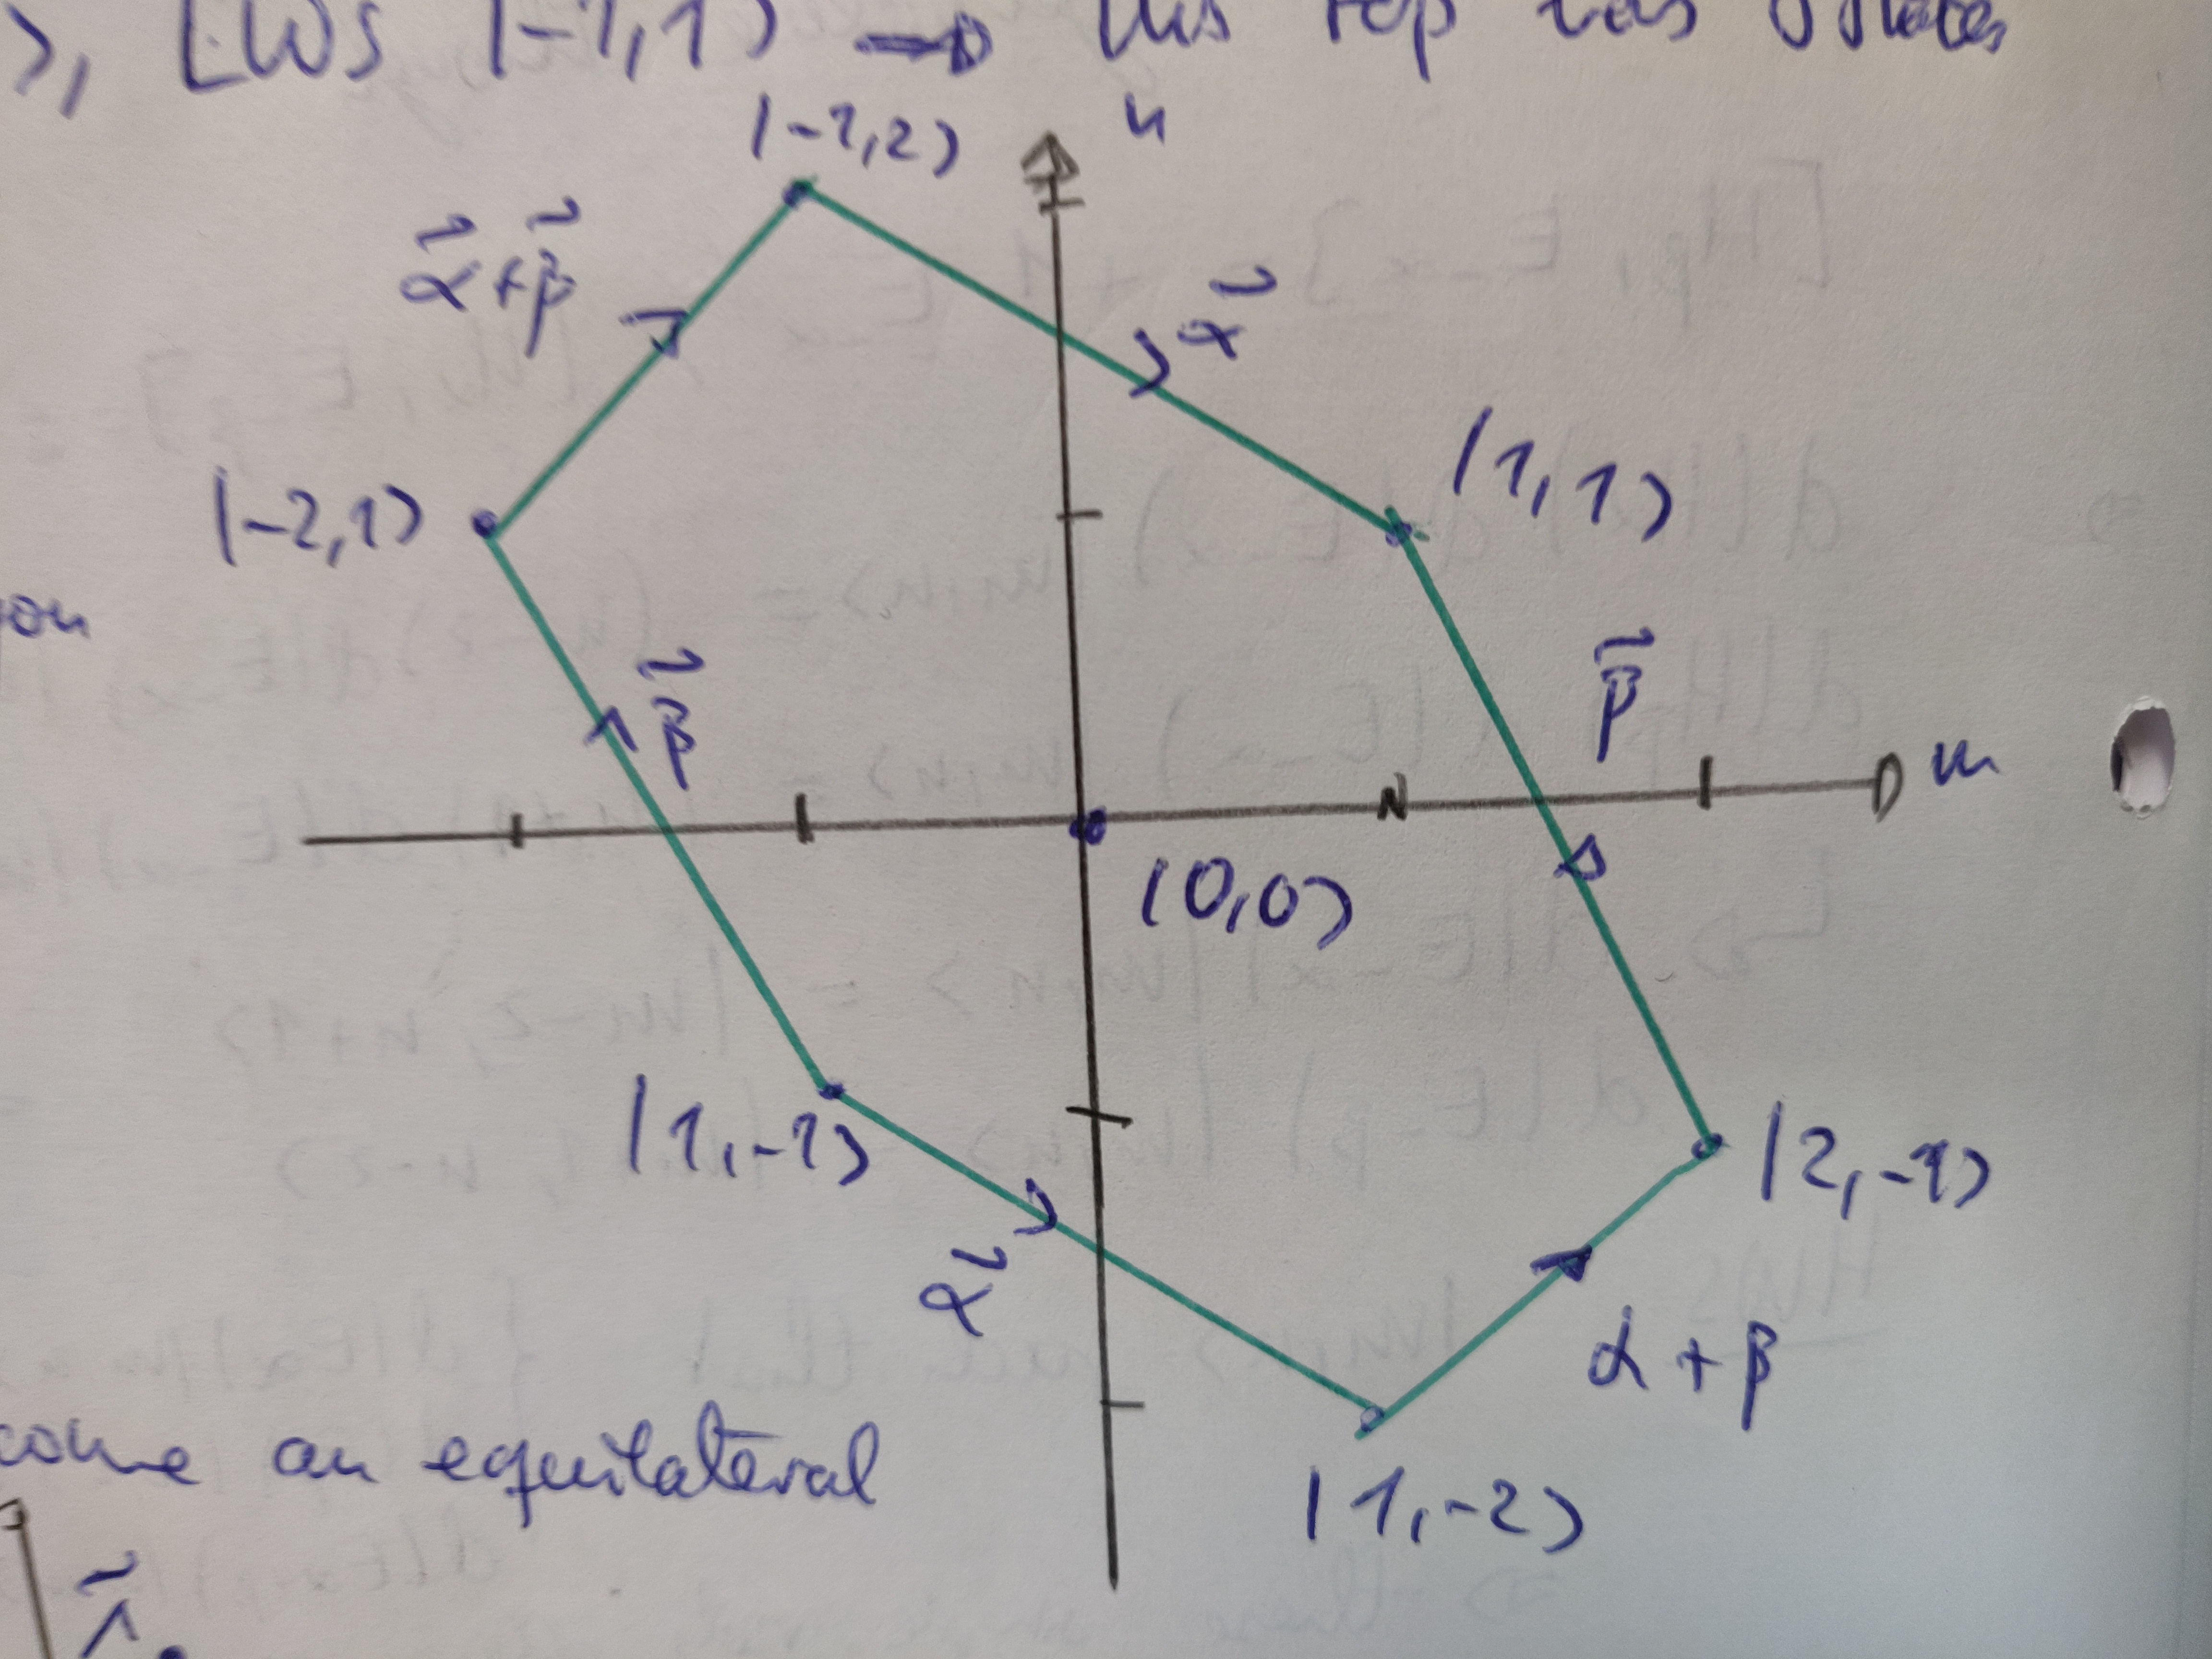
\includegraphics[width=0.5\linewidth]{gfx/squashedhexagon}
	\caption{}
	\label{fig:squashedhexagon}
\end{figure}
such that there is a non-trivial metric on this space of weights.
\\
Under a change of basis, the metric becomes standard Euclidean and in these coordinates we have the $\yng(2,1)$ rep becoming regular hexagon denoting $\Lambda$ as the HWS
\begin{figure}[h!]
	\centering
	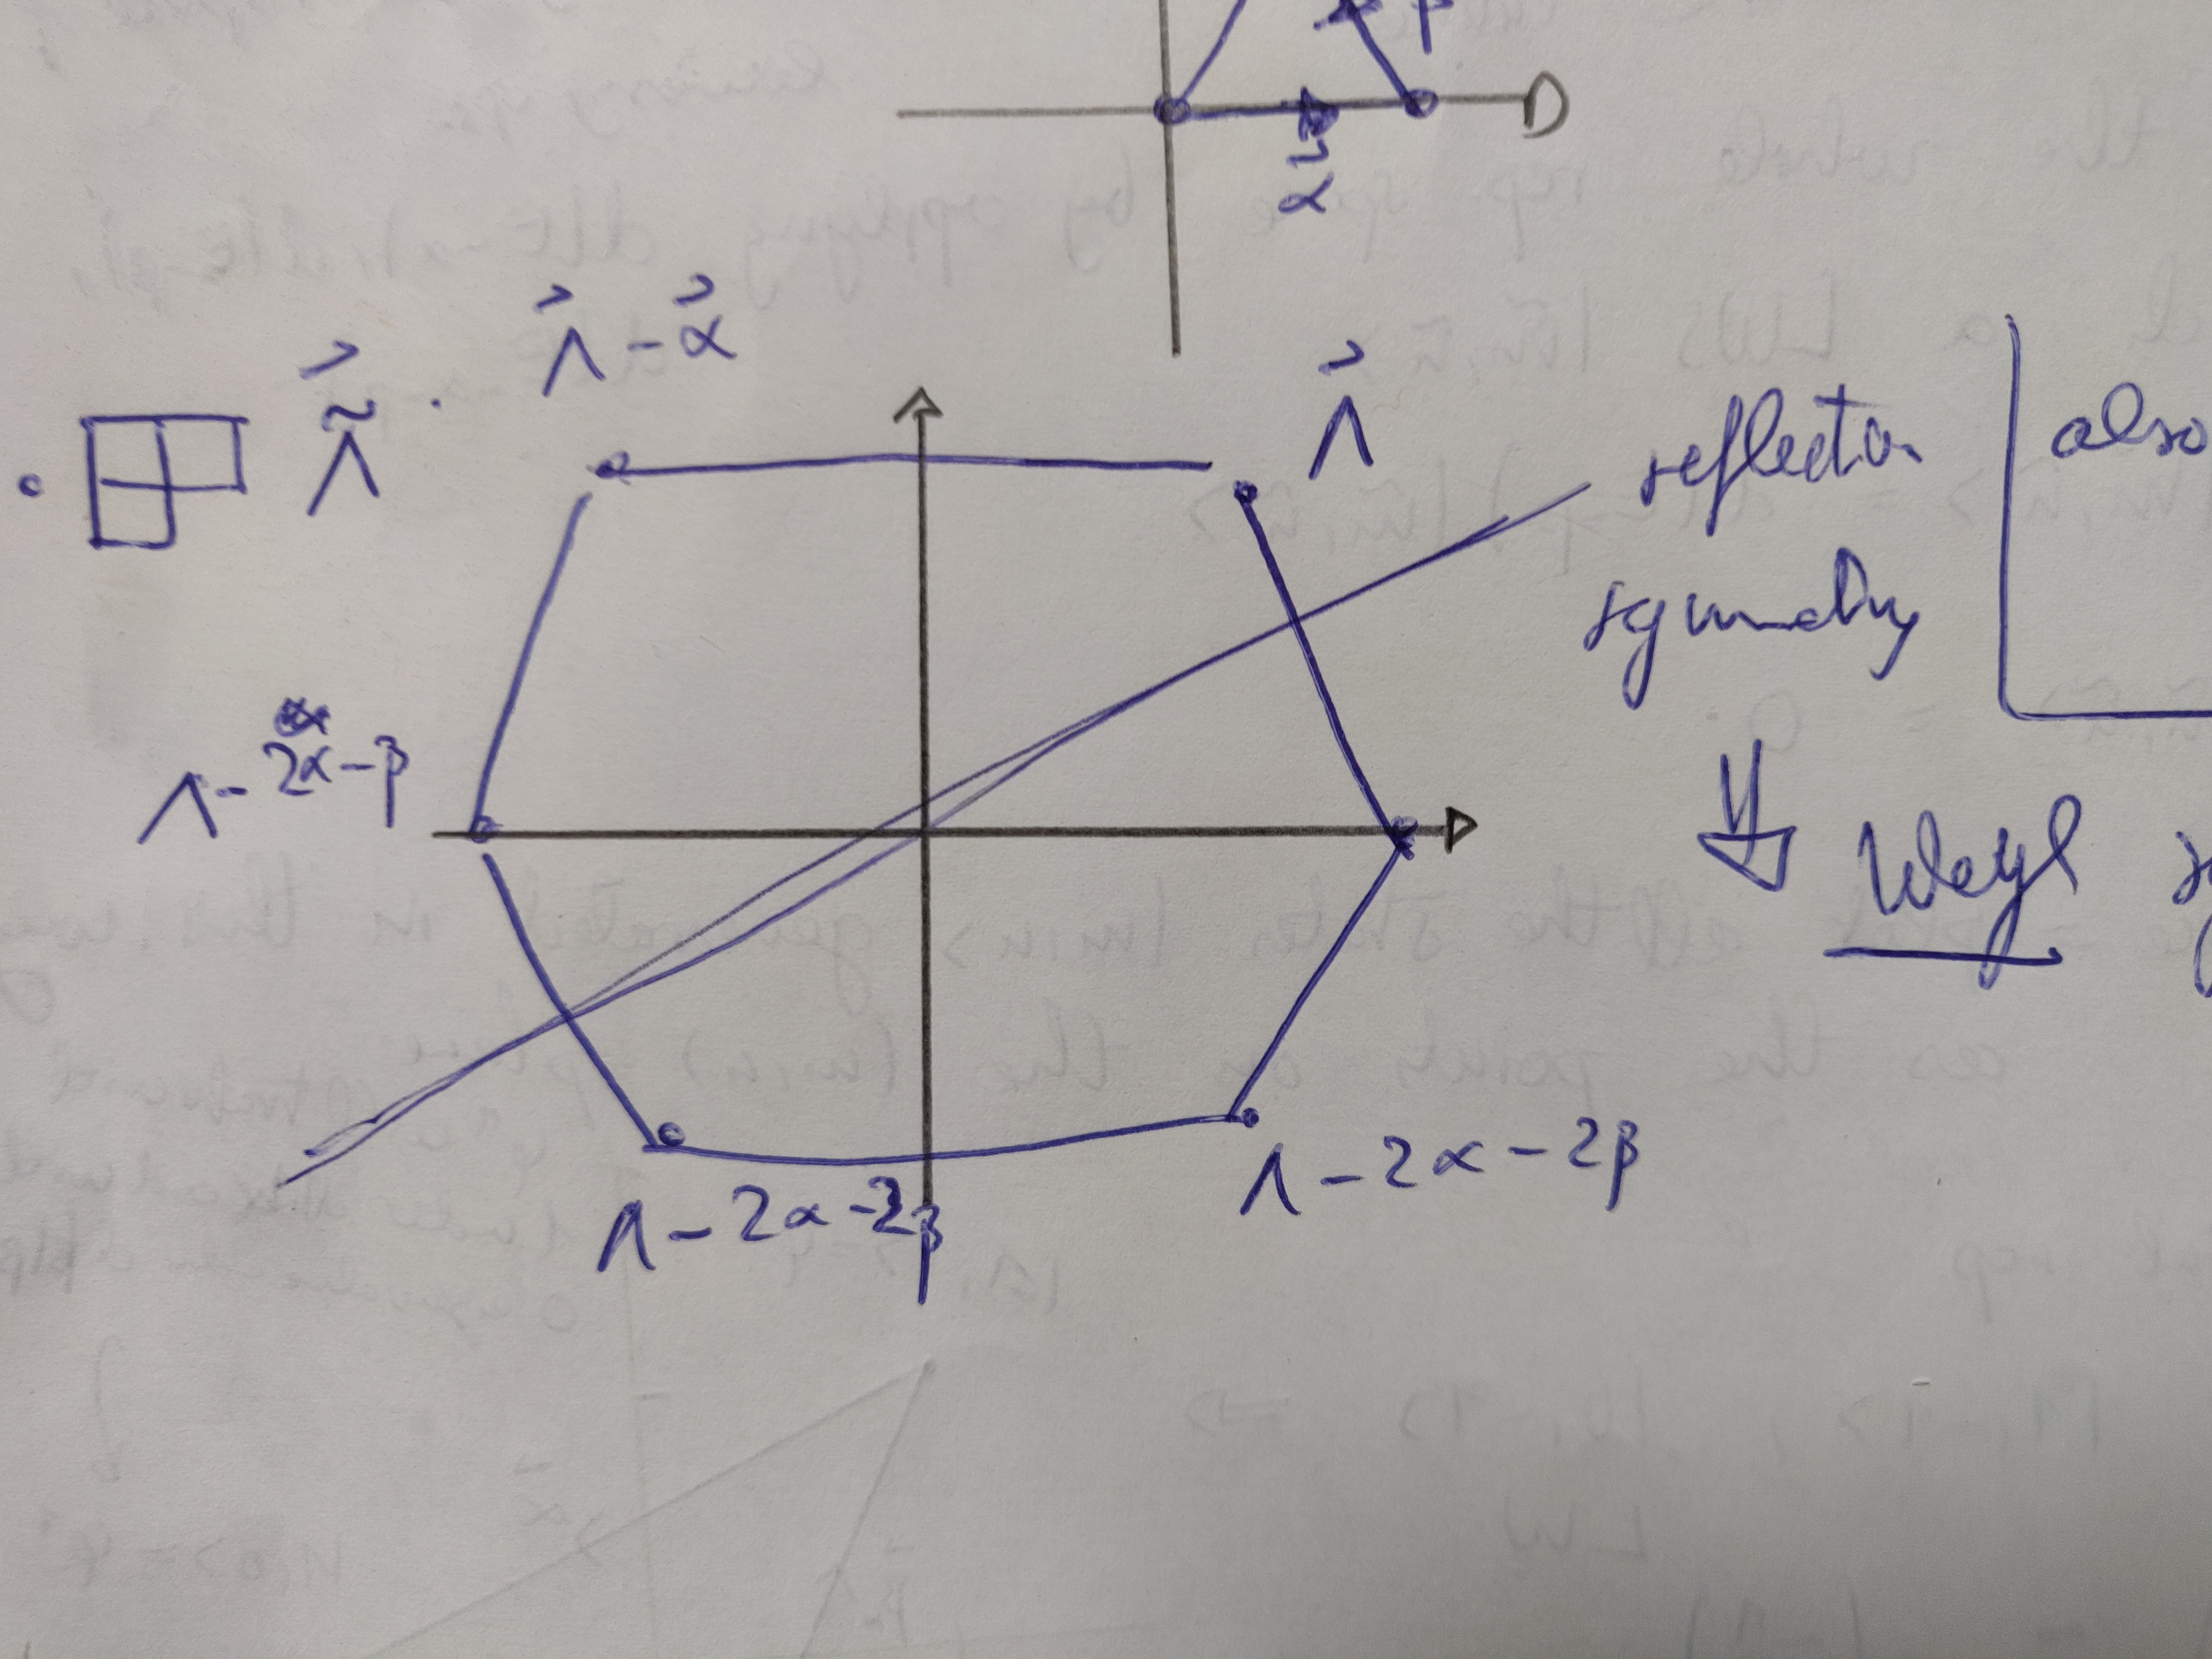
\includegraphics[width=0.5\linewidth]{gfx/weylsymmetrygroups}
	\caption{}
	\label{fig:weylsymmetrygroups}
\end{figure}
\end{enumerate}
\marginpar{General context: $\ket{m,n}$$\leftrightarrow$ Isospin+hypercharge (baryon number+strangeness), two quantum numbers which are conserved in combination (but also independently ?)}
Now for the transition into particle physics, the \emph{Eightfold way} postulated that isospin and strangeness are (actually not) independently conserved, i.e. it represents a symmetry of nature being arranged in irreps of some group falling into $(I_3,s)$ plane. Furthermore, for some spin particle with same baryon number were almost degenerate in mass (Schur's lemma !), one thought that quantum number being conserved (almost in reality) and same mass (almost in reality) one should have a symmetry corresponding to this, the resulting lattice is called the meson octett or the \emph{Eightfold way}.\\
Putting the third component of the isospin on the $x$-axis and the hypercharge (baryon number plus strangeness) on the $y$-axis, i.e. $H_\alpha \leftrightarrow \gamma,H_\beta \leftrightarrow I_3$ one gets
\begin{figure}[h!]
	\centering
	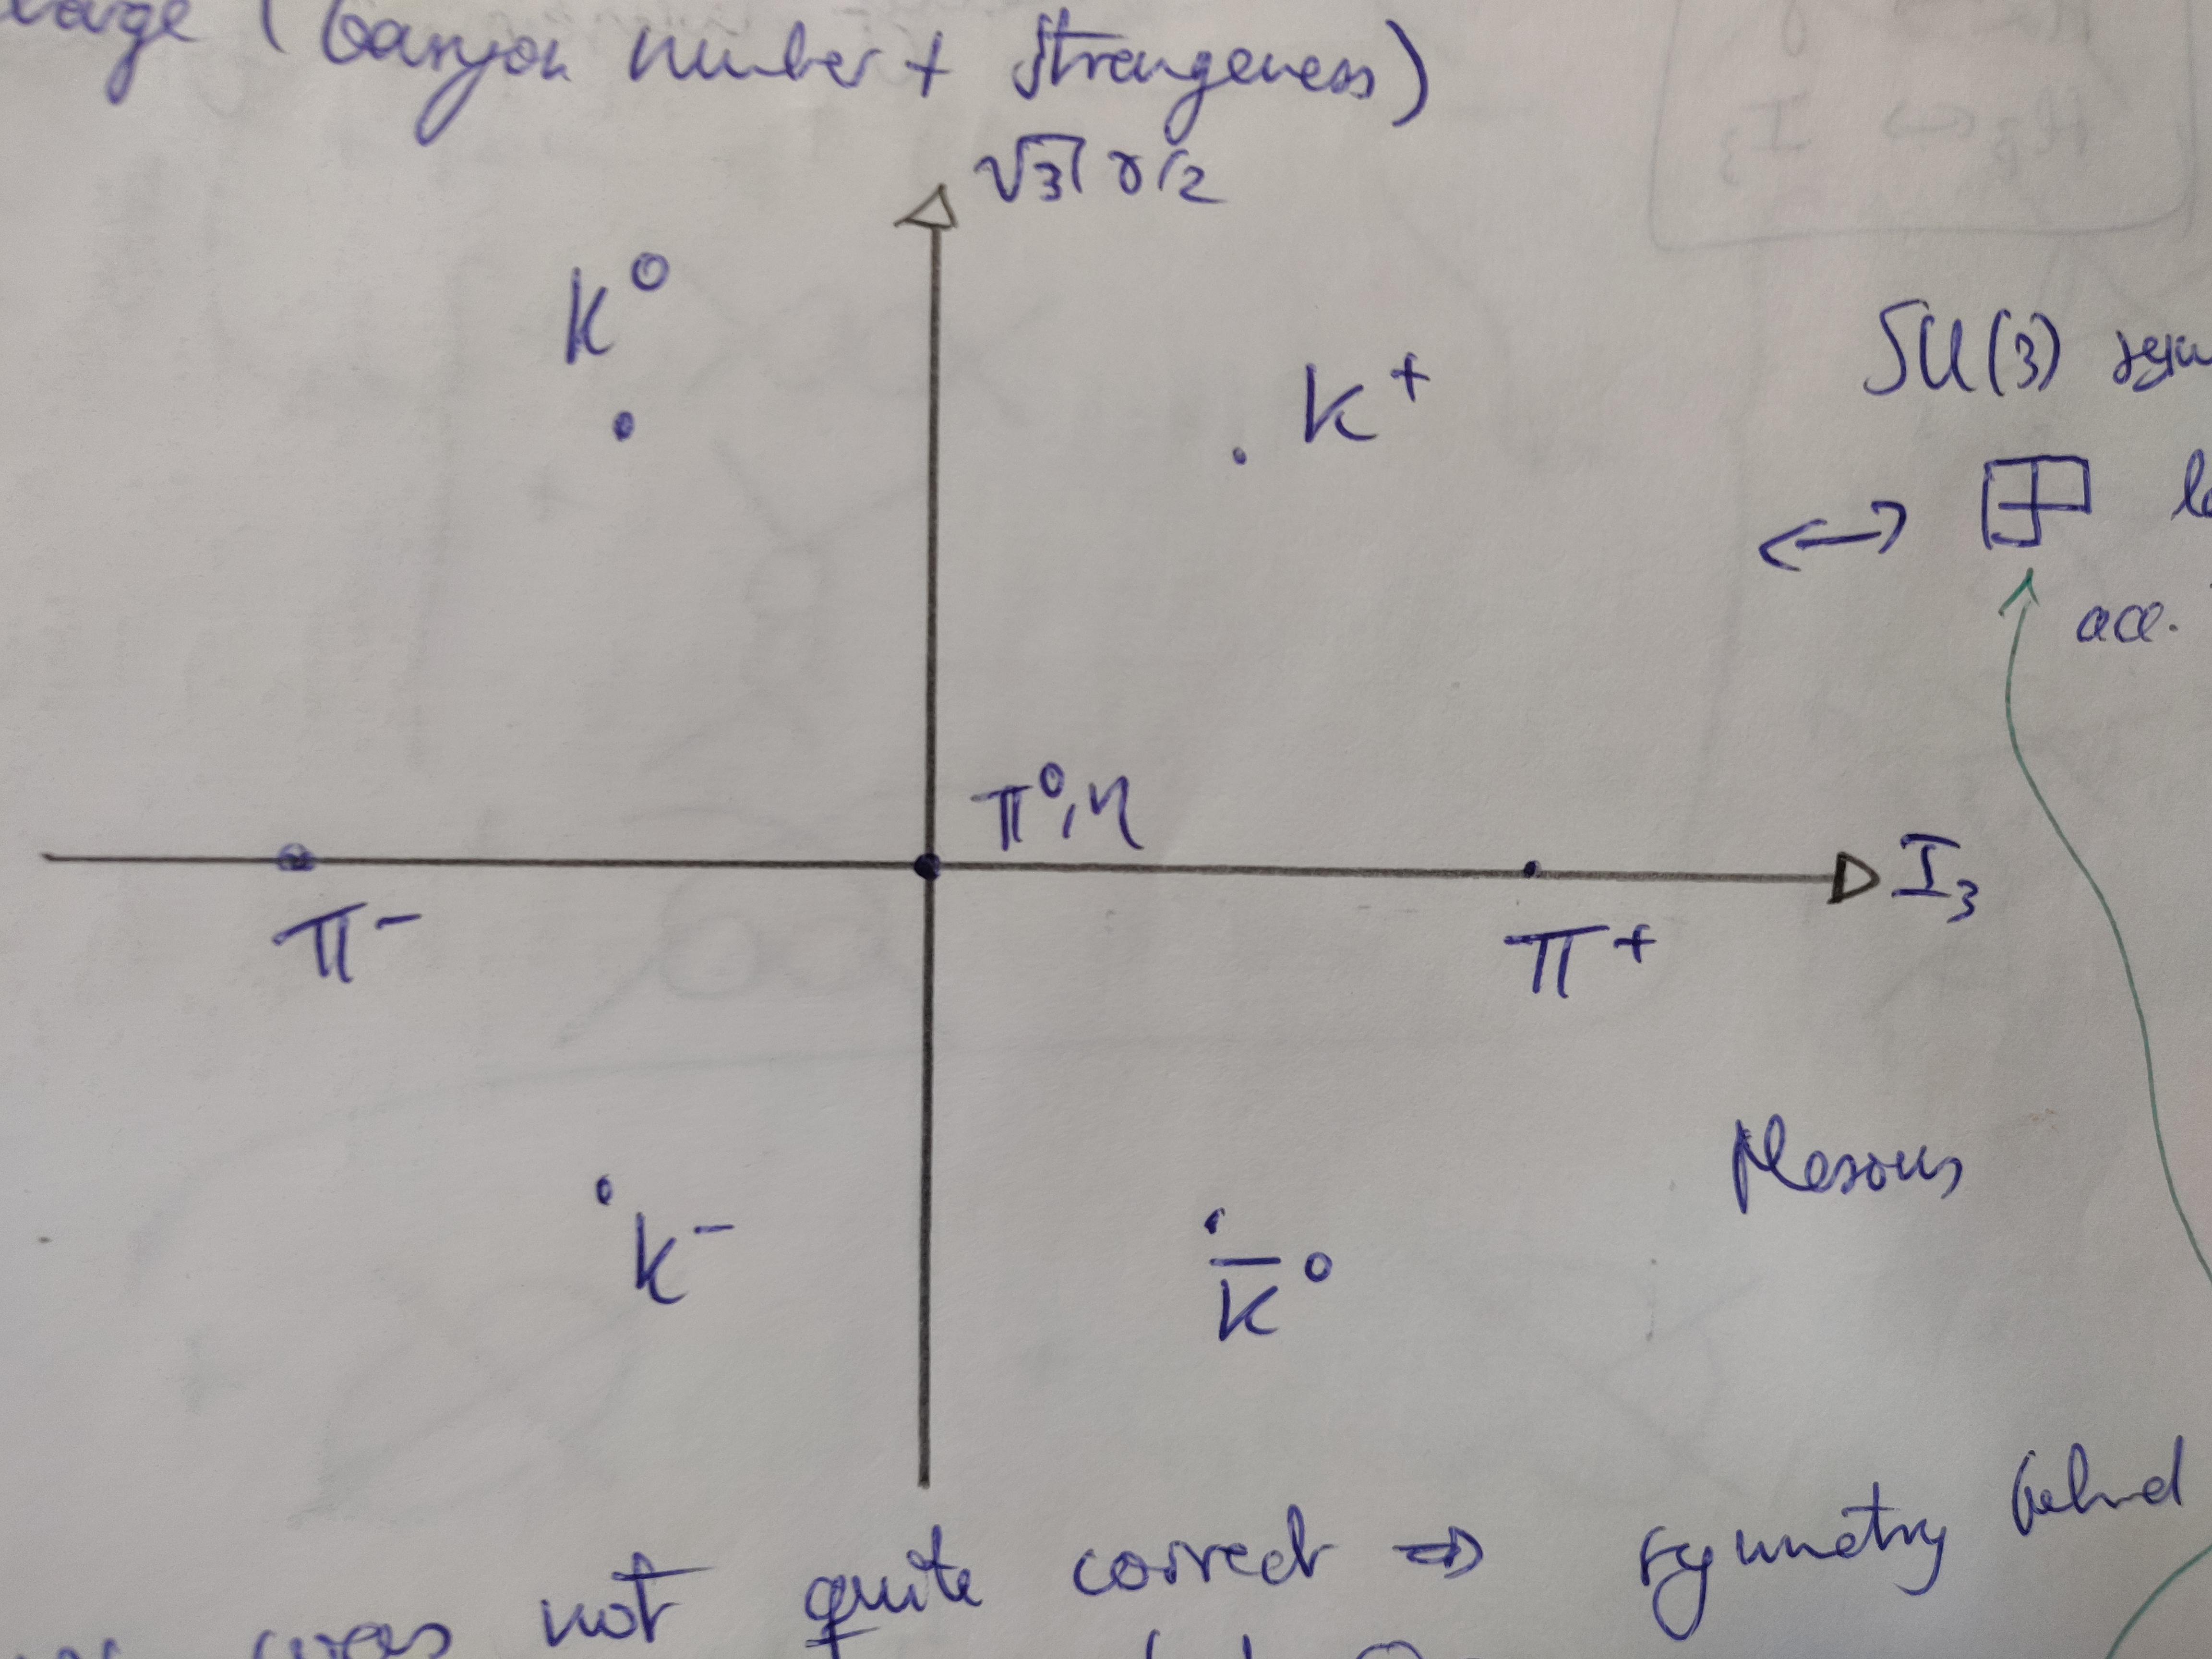
\includegraphics[width=0.7\linewidth]{gfx/eightfoldway}
	\caption{}
	\label{fig:eightfoldway}
\end{figure}
Presumably this corresponds to an $SU(3)$ symmetry, this diagram is equal to $\yng(2,1)$. However, this was not quite correct, the symmetry behind this arrangement wasn't hypercharge or Isospin, but rather QCD.\\
Mesons and Baryons:\\
Idea is that we have quarks $q \leftrightarrow \yng(1)$ transforming in the fundamental representation of $SU(3)$ and anti-quarks $p \leftrightarrow \bar{ \yng(1)}$ transforming in the anti-fundamental rep of $SU(3)$
\begin{align*}
	\text{Meson} &= \yng(1) \otimes \bar{ \yng(1)} = \yng(1) \otimes \yng(1,1) = \yng(2,1) \oplus \mI,\\
	\text{Baryon} &= \yng(1) \otimes \yng(1) \otimes \yng(1) = \yng(3) \oplus \yng(2,1) \oplus \yng(2,1) \oplus \mI \\
	\Leftrightarrow \quad 3\otimes 3\otimes 3&= \underbrace{10}_{\text{baryon decouplet}} \oplus \underbrace{8}_{\text{octett}} \oplus \underbrace{8}_{\text{octett}} \oplus \underbrace{1}_{\text{singlett}}\\
	&=
\end{align*}
\begin{figure}[h!]
	\centering
	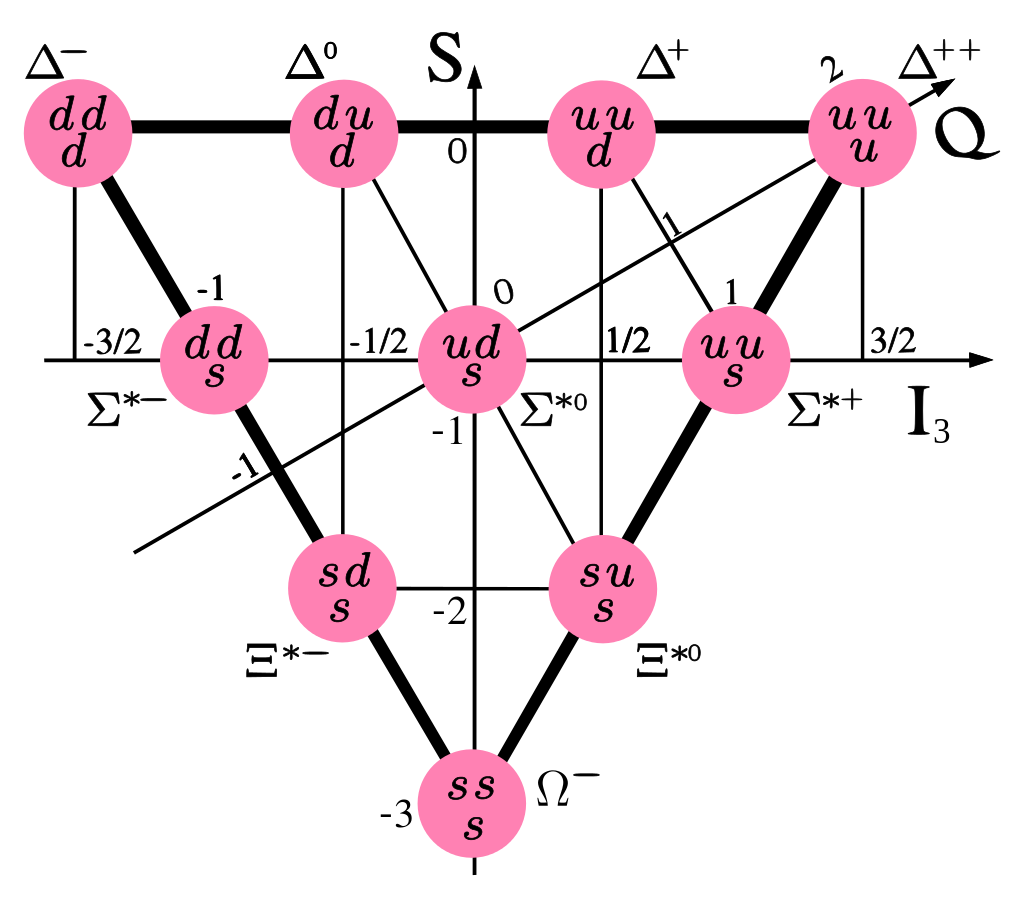
\includegraphics[width=0.5\linewidth]{gfx/Baryon-decuplet}
	\caption{}
	\label{fig:baryon-decuplet}
\end{figure}
note that each of these multiplets have different mass (Schur's lemma) as the symmetry is not really conserved.












\subsubsection{Connection of representation of Lie group at the example of $so(1,3)$ as in the chapter before}
The general idea is:\\
We have a Lie group, e.g. $SO(1,3)$, representing some property/symmetry (eg. spin) or our system, then the objects of our systems (i.e. particles) which have this property (i.e. $s=\half,1,\dots$) transform under irreducible representations of this group (scalar, vector/fundamental, pseudoscalar,pseudovector, tensor,\dots) where the irreducible representations are built via a combination from the generators of the corresponding Lie algebra, i.w. the $4\times 4$ generators $J^{\mu \nu}$ of $so(3,1)$.\\
\\

Consider the relation between matrix groups and Lie algebras: The map "exp" is a diffeomorphism of a small neighbourhood of $O \& \mathcal{I}$ in $M_{n\times n}(\mR)$ and $GL(n,\mR): \exp(a)=g,\exp(0)=\mathcal{I}$.\\
Lie($G$) is the linear subspace of $M_{n\times n}(\mR)$ generated by $exp^{-1}(O_{\mathcal{I}} )$, where $O_{\mathcal{I}}$ is a neighbourhood of $\mathcal{I}\in G \subset M_{n\times n}(\mR)$, compare \ref{fig:liegroups}. 
\marginpar{E.g. $G=SO(3)$, Lie(G)=$\{antisymmetric \, 3\times 3\, matrices\} \Rightarrow$ If $R=\exp(T)$, then $RR^T=e^T(e^T)^T =e^T e^{-T} = \mathcal{I}$.}
\begin{figure}
	\centering
	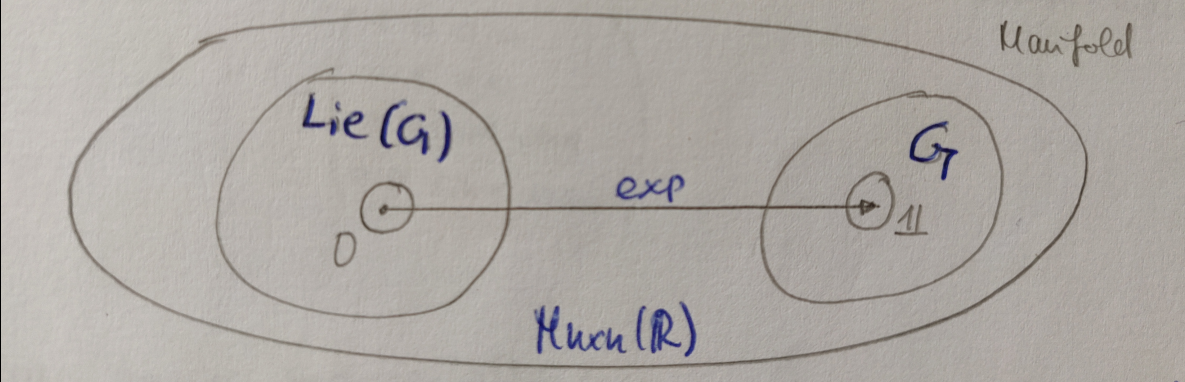
\includegraphics[width=0.7\linewidth]{gfx/Liegroups}
	\caption{\itshape Lie groups relation.}
	\label{fig:liegroups}
\end{figure}
$\Rightarrow exp(a)=g, a\in Lie(G), g\in G$ maps a small neighbourhood/patch of Lie(G) near $O$ to a small patch of $G$ near $\mathcal{I}$. If $a,b \in Lie(G)$, then 
$\exp([a,b])\in G$.
\begin{mybox}{Representation of a Lie-algebra}	
	\begin{equation}
	Lie(G) \stackrel{R}{\rightarrow} M(n), \quad a\mapsto R(a),
	\end{equation}
	with
	\begin{equation}
	R(0)=0, R([a,b])=R(a)R(b) -R(b)R(a) = [R(a),R(b)].
	\end{equation}
	Crucial:\\
	Given some representation $R$ of Lie-algebra Lie(G), we can always construct an associated representation of G (we call it also R) such that
	\begin{equation}
	R(A) = exp(R(a)) \quad if\quad A=\exp(a).
	\end{equation}
	Thus by having a representation of an element of Lie(G) 
	\begin{equation}
	w \, \Rightarrow \, w^{\nu} _{\mu}= -i \half \Omega_{\rho \sigma} (J^{\rho \sigma} )^{\nu}_{\mu} 
	\end{equation}
	we find a representation for an element of G
	\begin{equation}
	\Lambda^{\nu}_{\mu} =\left[\exp(-i \half \Omega_{\rho \sigma} (M^{\rho \sigma} ))\right]^{\mu}_{\nu}.
	\end{equation}
\end{mybox}
Consider $(J^{\rho \sigma})^{\nu}_{\mu}$ as the \emph{canonical basis} of so(1,3), thus these are the antisymmetric generators of SO(1,3). For $\Lambda \in SO(1,3)$ we find a $\tilde{\omega}$ such that we have a representation
\begin{align}
	\Lambda &= e^{\tilde{\omega}} \rightarrow \; \Lambda^{\;\nu}_{\mu} = \delta^{\nu}_{\mu} + \omega^{\nu}_{\mu} \\
	\omega^{\nu}_{\mu} &= -i \half \Omega_{\rho \sigma} (J^{\rho \sigma})^{\nu}_{\mu}.
\end{align}

\section{Lorentz group $SO(3,1)$ structure and Poincaré group}

\begin{mybox}{Poincaré group}
	The Poincarégroup $\mathcal{P}$ and the Lorentz group $L$ are made up of $L^\uparrow_+$, parity transformations $P$, time inversion $T$ and the translations $T_4$ in $\mathbb{M}^4$:
	\begin{equation}
	\label{eq:lorentzgroupwhole}
	L = L^\uparrow_+ \oplus T \oplus P,
	\end{equation}
	\begin{equation}
	\label{eq:poincaregroup}
	\mathcal{P}=L^\uparrow_+ \oplus T_4.
	\end{equation}
\end{mybox}

\subsection{Principle of relativity in the Lagrangian formalism }
\begin{mybox}{Principle of relativity take two}
	In order to obtain equations of motion whose form is the same for all observers, we demand:
	\begin{equation}
	\mathrm{The\, Lagrangian \; \mL \;of \;a \;relativistic\; FT\; is\; invariant \;under \;\mathcal{P}^\uparrow_+}.
		\end{equation}
		Equations that are form invariant are called \emph{covariant}.
	\end{mybox}
	Note the restriction to $\mathcal{P}^\uparrow_+$. Always keep this restriction in mind when reading ’Lorentz invariance’.
	\\
	\\
	This postulate immediately guarantees that the Euler-Lagrange equations are Lorentz covariant
	and that quantities derived from L in a covariant way are Lorentztensors.
	In anticipation of the standard model it should be noted that nature really is not described by a
	Lagrangian that is invariant under parity or timeinversion transformations and we will use terms
	violating P and T when building our SM Lagrangian so excluding those here is really necessary.
\subsection{Generators of boosts and rotations in Minkowski space}

























\subsection{Representation of the Lorentz group}
\label{subsec:repLorentzgroupPhysics}
We want a theory satisfying SRT, this is only satisfied if all fields transform in an irrep of the Lorentz group. Then we will have to study different types of reps (scalar, vector, spinor,\dots) and look at their Noether current wrt. spatial rotation, which has orbital and spin contributions, from which we can read off which spin corresponds to which representation. Thus, \textbf{spin is an afterthought, not an input for the theory}. First we study reps and then afterwards we can make the identification with particles and spin.\\
\\
Relativistic fields are classified by their behaviour under Lorentz transformations, i.e a general transformation
\begin{equation}
	D(\Lambda): \varphi(x) \rightarrow \varphi^\prime (x^\prime) = D(\Lambda) \circ \varphi(x),
\end{equation}
where $D(\Lambda)$ is a particular representation of the element $\Lambda$ of the Lorentz group and where the Lorentz four-vector transforms in a particular representation, namely the vector representation
\begin{equation}
x^{\mu} \mapsto x^{' \mu} = \Lambda^{\mu}_{\nu} x^{¸\nu}, \quad \Lambda^{\mu}_{\nu} \in SO(1,3).
\end{equation}
Generally a field $\phi^a(x)$ transforms then as a representation of the \emph{Lorentz group} $SO(1,3)$. With the field being a map
\begin{equation}
\phi^a :\mR^{1,3} \rightarrow V, x\mapsto \phi^a(x), \; a=1,\dots, \dim V=n
\end{equation}
we have
\begin{equation}
\phi^a(x) \mapsto \phi^{'a} (x) = D(\Lambda)^a_b \phi^b (\Lambda^{-1} x') = D(\Lambda)^a_b \phi^b(x)
\end{equation}
with $D(\Lambda)$ being the representation for $\Lambda \in SO(1,3)$.
\subsubsection{Collection of the different representations of the Lorentz group - a physical approach}
\begin{enumerate}
	\item \emph{Scalar representation}:\\
	
		For a real/complex scalar ($s=0$) field $\phi(x)$, the representation is trivial 
	\begin{equation}
	D(\Lambda) = \mathcal{I} \quad \forall \Lambda \; \Rightarrow \phi'(x')=\phi(x).
	\end{equation}
	This representation only has one dof., it turns out to describe (via angular momentum Noether current) bosons of spin $s=0$.
	\item \emph{Vector representation}:\\
		A vector field ($s=1$) $A^{\mu}(x)$ transforms in the \emph{vector representation} 
	\begin{equation}
	D(\Lambda) = \Lambda^{\;\nu}_{\mu} \quad \forall \Lambda \; \Rightarrow A_{\mu}(x)\rightarrow A^\prime_\mu(x^\prime) = \Lambda^{\;\nu}_\mu \underbrace{A^{\nu}(\Lambda^{-1}x' )}_{=A^\nu(x)}.
	\end{equation}
	From the angular momentum Noether current we know that the Vector rep describes spin $1$ particles (and anti-particles). Spin $1$ has $3$ polarizations ($-1,0,1$), i.e. one longitudinal and two transvere degrees of freedom.\footnote{You can combine the transverse polarizations $T_{1,2}$ to $T_1\pm i T_2$ to describe left-and right-handed polarizations.} Thus, for a vector we do expect $4$ degrees of freedom, but it has $\mu=0,1,2,3 \Rightarrow 4$. The one redundant degree of freedom is fixed by the gauge (as vector fields are gauge fields). Gauge fields have unphysical degrees of freedom corresponding to gauge transformations which can be removed by fixing the gauge transformation. Thus, there is another symmetry beside the Lorentz symmetry in this system under which the vector gauge fields transform, namely the \emph{gauge symmetry}. Gauge fixing, e.g. $\partial_\mu A^\mu=0$, $A_0=0$, removes one dof. such that only $3$ survive.\\
	 However, the photon field only has $2$ polarizations, what happens with the $3$rd ? It decouples. Unbroken gauge invariance (like QED) implies that $m_{\text{gauge field}}=0$, a \textbf{mass term would break gauge invariance}. Whenever $m_{A_\mu}=0$, then the longitudinal polarization decouples, only two dof $\gamma^\pm$ are left, namely the $2$ transverse polarizations.\\
	 Examples of Vector theories:\\
	 \begin{enumerate} 
	 \item Thus, QED is a $U(1)$ gauge theory, the vector field $A_\mu$ gives rise to photons $\gamma$ with $+,-$ transverse polarizations only and $m_\gamma=0$.\todo{Reference to this theory}
	 \item QCD is a $SU(3)$ gauge theory, the vector field $A^{a=1,\dots,8}_\mu$ are $8$ gluon fields (as $SU(3)$ has $8$ generators) $g^{1\dots 8}$ which are also massless, because it has an exact gauge symmetry, $m_g=0$ with two polarizations.\todo{Reference to this theory}
	 \item Weak interactions are described by $SU(2)_L$ gauge theory (Glashow-Weinberg-Salam), the weak interaction sector of the standard model. $SU(2)$ has $3$ generators, which implies that there exist $3$ vector fields $A^{a=1,2,3}_\mu$ which actually are the $3$ weak vector bosons $W^+,W^-,Z^0$ \todo{reference to this theory}. However, these \emph{are massive} $m_{W^\pm}\neq 0, m_{Z^0}\neq 0$, because the $SU(2)$ gauge symmetry is spontaneously broken by the Higgs mechanism. Thus, there are $3$ spin polarizations for each $W^+,W^-,Z^0$, i.e. $1$ longitudinal $L$ and two transverse $+,-$.
	 \end{enumerate}
 \item \emph{Tensor representation}:\\
 A rank $(0,2)$ tensor transforms according to 
 \begin{equation}
 T\munu(x) \rightarrow T^\prime\munu(x^\prime) = \Lambda^{\;\rho}_\mu \Lambda^{\;\sigma}_\nu T_{\rho \sigma}(x).
 \end{equation}
 Rank $(0,2)$ tensors are however reducible, they decompose into two irreps, i.e. the \emph{symmetric} and \emph{anti-symmetric} irrep. Whilst the symmetric tensor irrep describes spin $2$ particles like the graviton, the antisymmetric tensor irrep does not describe any new particles as it can be constructed from vectors, consider for example the field strength $F\munu =\partial_\mu A_\nu - \partial_\nu A_\mu$, i.e. not an independent degree of freedom.\\
 \\
 \textbf{Renormalizability of QFT} is the essential requirement which confines our interest to the scalar, vector and spinor representation, as e.g. the symmetric $2$ tensor rep represents a non-renormalizable theory, i.e. gravity.
 \item \emph{Lowest spinor representation}:\\
 A spinor like the Dirac fermion/spinor field $\psi_D(x)$, which is a four-component complex-valued spinor, transforms in the spinor representation
 \begin{equation}
 	D(\Lambda) = S \in M^{4 \times 4}, \; S=S(\gamma^\mu) \Rightarrow \; S\circ \psi_D(x).
 \end{equation}
 A (Dirac) spinor is not a vector as it does \emph{not} transform like a vector but like a spinor (i.e. $4\pi$ rotation to identity).\\
 It is a reducible rep made up out of $2$ irreps
 \begin{enumerate}
 	\item $\psi^{\alpha=1,2}_L$ is the left-handed irrep for the \emph{Weyl spinor}, which is a $2$-component spinor $\alpha=1,2$.
 	\item $\psi_{R,\dot{\alpha}=1,2}$ is the right-handed irrep for the Weyl spinor, which is a $2$-component spinor $\dot{\alpha}=1,2$
 \end{enumerate}
In the \emph{Chiral basis} for $\gamma^\mu$, i.e. 
\begin{equation*}
	\gamma^\mu = \begin{pmatrix}
	0&\sigma^\mu \\ 
	\bar{ \sigma}^\mu &0\\
	\end{pmatrix}, \quad \sigma^\mu =(\mI,\vec{\sigma}), \quad \bar{ \sigma }^\mu =(\mI,-\vec{\sigma}),
\end{equation*}
the Dirac spinor decomposes into the two Weyl spinors
\begin{equation}
\psi_D(\begin{pmatrix}
\psi^\alpha_L\\ \psi_{R,\dot{\alpha}} \\
\end{pmatrix})
= \begin{pmatrix}
\psi^1_L\\
\psi^2_L\\
\psi_{R,\dot{1}} \\
\psi_{R,\dot{2}} \\
\end{pmatrix}
\end{equation}
where the respective indices of the disjoint subspaces $(\sigma^\mu)^{\alpha \dot{\alpha}}$, $(\bar{ \sigma }^\mu)_{\dot{\alpha}\alpha}$, $\;\alpha,\dot{\alpha}=1,2$ are raised and lowered with $\epsilon$ tensors $\epsilon^{\alpha \beta}, \epsilon_{\dot{\alpha}\dot{\beta}}$ respectively.\\
\\
Note that there are also LH and RH electrons which we group into the Dirac electro ($\leftrightarrow\psi_D$) as they interact the same way with photons and gluons. However, they interact differently with $W^\pm$. Thus, the electron as an elementary particle is not corresponding to a reducible rep, i.e. $\psi_D$, but really corresponds to the $2$ irreducible Weyl spinor $e^-_L,e^-_R$.\\
$\psi_L$ describes LH chiral fermions (i.e. chirality is $+\half$) whereas $\psi_R$ describes RH chiral fermions with chirality $-\half$. They do transform differently under $SO(1,3)$ where they have different signs in the boost \ref{subsubsec:lhrhSpinors}.
\end{enumerate} 



\subsection{The Lorentz group $SO(1,3)$}
\subsubsection{Lorentz group structure}
\begin{mybox}{Proper Lorentz group}
	The set of proper (Lorentz trafo is called proper if $\det\Lambda=1$ holds for its representation), orthochronous (Lorentz trafo is called orthochronous if $\Lambda^0_0 \geq 1$ holds true for its representation) Lorentz transformations makes up the six dimensional Lorentz group
	\begin{equation}
	\label{eq:lorentzgroup}
	L^\uparrow_+ :=\left\{	\Lambda| \eta\munu\Lambda^\mu_{\;\rho} \Lambda^\nu_{\;\sigma} = \eta_{\rho \sigma}, \; \Lambda^0_0 \geq 1,\; \det(\Lambda)=1\right\}.
	\end{equation}
	Note that 
	\begin{equation}
	L^\uparrow_+ = SO(3,1).
	\end{equation}
	It is a subgroup of the Lorentzgroup of which every element is countinously expandable from $\Lambda=\mI$.
\end{mybox}
Equivalent notations of the equation in \ref{eq:lorentzgroup} are
\begin{align}
	\Lambda^{\mu \rho} \Lambda_{\mu \sigma} &= \delta^\rho_\sigma \\
	\Lambda^{\;\rho}_\mu \Lambda^\mu_{\;\sigma} &= \eta^\rho_\sigma.
\end{align}
\begin{mybox}{Basis of $\mso(1,3)$}
	The Lorentz group is generated by six antisymmetric $4\times4$ matrices, the basis of the six-dimensional Lorentz algebra $\mso (1,3)$
	\begin{equation}
	(J^{\rho  \sigma})^{\mu \nu} = i \left[\eta^{\rho \mu} \eta^{\sigma \nu} - \eta^{\rho \nu} \eta^{\sigma \mu} \right].
	\end{equation}
	This is the algebra of infinitesimal Lorentz transformations connected to the identity. We find in this basis
	\begin{equation}
	\Lambda^{\mu}_{\nu} = \left[e^{-i \half w_{\rho \sigma }J^{\rho \sigma}  }\right]^{\mu}_{\nu}.
	\end{equation}
	The defining commutator of the Lie-algebra $\mso(1,3)$ is 
	\begin{equation}
	\label{eq:commutatorso3}
	[J^{\mu \nu}, J^{\rho \sigma} ] = i \left[\eta^{\nu \rho} J^{\mu \sigma} - \eta^{\mu \rho} J^{\nu \sigma} - \eta^{\nu \sigma} J^{\mu \rho} + \eta^{\mu \sigma} J^{\nu \rho}\right].
	\end{equation}
	These six basis elements $(J^{\rho \sigma})^{\mu \nu}$ therefore generate the three boosts and three rotations of the Lorentz group SO(1,3).
\end{mybox}
We can set
\be 
\label{eq:lorentzGeneratorRotationsBoosts}
J_{ij}=\epsilon_{ijk} J_k \qquad, \; J_{0i}=K_i,
\ee 
where $J_k$ is the generator of rotations and $K_i$ is the generator of boosts.
The group of rotations is compact, i.e. the generators are hermitian $J=J^\dagger$, whilst the group of boosts is non-compact, i.e. the generators are anti-hermitian $K^\dagger=-K$.\footnote{This is due to the fact that $\beta \in [0,\infty)$, we can not boost to infinity. This is explained in more detail below.}
Then
\be
[J_i,J_k] = i \epsilon_{ijk} J_k, \quad [J_i,K_k] = i \epsilon_{ijk} K_k,\quad [K_i,K_j] = - i \epsilon_{ijk} J_k.
\ee

\subsubsection{New basis of $SO(1,3)$ to find irreducible representations}

We can now change basis in order to find the irreps. later on. We complexify $\mso(1,3)$ to $\mathfrak{sl}(2,\mathbb{C})$ by changing to the new basis operators
\bse 
\Vec{J}^\pm = \frac{1}{2}(\Vec{J}\pm i \Vec{K}),
\ese 
which are hermitian. This is useful because we then have have disjoint, i.e. separate $\msu(2)$ subalgebras for $+,-$ respectively, i.e. $\msu(2)_L$ and $\msu(2)_R$
\be
[J^+_i, J^+_j] = i \epsilon_{ijk} J^+_k,\qquad [J^+_i,J^-_j]=0.
\ee 
Later on we will get the irreducible representations of $SO(1,3)$ be deducing the irreps. of $\msu(2)_{L,R}$.
Now we can label the irreps of the Lorentz group via this decomposition by two half-integers $(s_+,s_-)$, where
\be 
(\Vec{J}^\pm)^2 = s_{\pm} (s_{\pm} + 1), \quad s_{\pm} \in \{0,\frac{1}{2},1,\dots\}=\left\{\frac{\Z}{2}\right\} .
\ee 
Note that by complex conjugation we swap the copies
\bse 
(s_+,s_-) \Longleftrightarrow (s_-,s_+),
\ese 
which is often indicated by writing
\be 
\mso(1,3) = \frac{\msu(2)\times \msu(2)^*}{\mathbb{Z}_2}.
\ee 
The $\Z_2$ quotient imposes that $SO(1,3)$ irreps have spin $s_+ + s_- \in \mathbb{Z}$. The object on the RHS which is quotiened is called spin-group $Spin(1,3)$, which is the double cover of the Lorentz group
\bse 
Spin(1,3) = SU(2) \times SU(2)^*.
\ese\footnote{$Spin(3)$ is the double cover of $SO(3)$ which is $SU(2)$}
The group is 
\be 
SL(2,\mC) = \left\{ M= \begin{pmatrix}a&b \\
	c&d\\
\end{pmatrix} | a,b,c,d \in \mC, \det M = ad-bc=1\right\}
\ee 




\subsection{Representations of the Lorentz group}
\label{subsec:lorentzrep}
\subsubsection{Explicit $\mso(3,1)$ representations}
In the new basis, we get two disjoint copies of $\msu(2)$, namely 
\be
\msu(3)=\msu(2)_L \times \msu(2)_R = (\half,0) \oplus (0,\half)
\ee 
 which, provided their irreps, give us the irreps of the Lorentz group. We know the irreps of $\msu(2)$ from \ref{subsubsec:irrepssu2} to be
 \bse 
 \cdot=\mI,\quad \yng(1),\quad \yng(2),\dots
  \ese 
  We just need an integer $s\in \mathbb{N}$ to specify an $\msu(2)$ irrep, i.e. for $\mso(3,1)$ we need two integers $(s_+,s_-)$.
   Now we can label the irreps of the Lorentz group via this decomposition by two half-integers $(s_+,s_-)$, where
  \be 
  (\Vec{J}^\pm)^2 = s_{\pm} (s_{\pm} + 1), \quad s_{\pm} \in \left\{0,\frac{1}{2},1,\dots  \right\}.
  \ee 
Any $SO(3,1)$ irreps $(s_+,s_-)$ $\rightarrow(\msu(2)_L,\msu(2)_R)$ has dimension
\begin{equation*}
	\dim(s_+,s_-) = (2s_++1)\cdot (2s_-+1).
\end{equation*}
The interesting possible irreducible representations of $\mso(3,1)$ are the following.
\marginpar{The maths convention is always a twice the value.}
\begin{enumerate}
\item[$(0,0)$] \emph{Trivial representation}, the scalar field $\phi$
\item[$(\half,0)$] \emph{Left-handed Weyl spinor} $\psi_\alpha$ ($\alpha=1,2$) which transforms in the fundamental representation of $\msu(2)_L$ and in the trivial rep of $\msu(2)_R$
\item[$(0,\half)$] \emph{Right-handed Weyl spinor} $\bar{ \psi}_{\dot{\alpha}}$ ($\dot{\alpha}=1,2$) which trafos as trivial rep of $\msu(2)_L$ and in the fundamental rep of $\msu(2)_R$.
\item[i)] Note that the Dirac spinor itself is not an irreducible representation but a composite of two irreducible reps, namely the left-and right-handed Weyl spinors
\begin{equation*}
	\text{Dirac spinor} = (\half,0) \oplus (0,\half) = \psi_D = \begin{pmatrix}
		\psi_\alpha\\
		\bar{ \psi}_{\dot{\alpha}}\\
			\end{pmatrix}
\end{equation*}
The Dirac spinor has the following dimensions
\begin{equation*}
 \dim\left[(\half,0)\oplus (0,\half) \right] = 4.
\end{equation*}

\item[$(\half,\half)$] \emph{Vector representation} for $A_\mu$, which transforms in the fundamental rep of $\msu(2)_L\&\msu(2)_R$.\\
How do we get to the vector representation $A_\mu$ when it should actually be $A_{\alpha \dot{\alpha}}$ ? Via repackaging:\\
Note that the dimensions are $\dim(\half,\half)=2\cdot 2=4$, i.e. a $4$-component vector, and that $\dim(\half,0)=\dim(0,\half)=2$, i.e. $A_{\alpha \dot{\alpha}}$ is a $2\times2$ matrix with $4$ components.
\item[$(1,0)$] \emph{Self-dual $2$-form} which is given by $F_{(\alpha \beta)}$, by repackaging one has eg. objects $F\munu= \half \epsilon{\munu \rho \sigma} F^{\rho \sigma}$, with $F_[\mu \nu], F=*F$, which is what one calls an \emph{instanton}.
\item[$(0,1)$] \emph{Anti-self-dual $2$-form} which is given by $B_{\dot{\alpha}\dot{\beta}}$, by repackaging one has eg. objects $B\munu= - \half \epsilon_{\mu \nu\rho \sigma} B^{\rho \sigma}$ with $B=-*B$, which is what one calls an \emph{anti-instanton}.
\end{enumerate}

\subsubsection{A comment on Left-handed vs Right-handed Weyl Spinors}
\label{subsubsec:lhrhSpinors}
\begin{enumerate} 
	\item[LH]
As described above, the LH Weyl spinor $(\half,0)$ transforms in fundamental rep $\yng(1)$ of $SU(2)_L$ and in the trivial rep $\mI$ of $SU(2)_R$, i.e.
\begin{equation*}
	(\half,0)=\yng(1)_L \times \mI_R.
\end{equation*}
Thus, the generators of $\msu(2)_L$ must be represented in fund rep: $\md(N_i)=-\half \sigma_i$, whereas the generators of $\msu(2)_R$ must be represented in scalar rep $\md(\bar{ N}_i)=0$. \\
Consider the group action of the LH spinor by considering one group element of $SO(3,1)$, $\Lambda^\mu_{\;\nu}=\exp(\omega^\mu_{\;\nu}), \omega^\mu_\nu$ has $6=r_i+b_i=3+3$ parameters, $3$ rotations $r_i$ and $3$ boosts $b_i$
\begin{equation*}
	D(\Lambda): \psi_\alpha \rightarrow \exp(\underbrace{n_i}_{Ar_i+Bn_i} \md(N_i))^\beta_\alpha \psi_\beta = \underbrace{\exp(-\frac{i}{2} r_i \sigma_i \textcolor{red}{-} \frac{b_i}{2}\sigma_i)^\beta_\alpha}_{M^\beta_\alpha}\psi_\beta
\end{equation*}
which is \emph{not} a unitary irreps, since $\sigma_i b_i$ is not a unitary matrix as $\sigma_i$ is only hermitian. Therefore $M^\beta_\alpha \in SL(2,\mathbb{C})$, which is the complexification of $SU(2)$. $SO(3,1)$ is a non-compact group since boost never reach $c$, only $v<c$ is allowed. If you picture Lie groups as manifolds, then the Lorentz group is not spherical but rather hyperbolically formed as $\beta \in (-1,1)$ such that the manifold is non-compact.\\
We only get a pseudo representation of $SO(3,1)$ as $r_i$ needs $4\pi$ to get back to identity. Therefore, \emph{spinors are just a pseudo-representation}, even though they are composite objects of real irreps.
\item[RH] Transforms in trivial rep of $\msu(2)_L, \tilde{\md}(N_i)=0$, and in the fundamental rep of $\msu(2)_R, \tilde{\md}( \bar{ N}_i)= - \frac{i\sigma_i}{2}$. Consider the group action under the same group element as above
\begin{align*}
	\tilde{D}(\Lambda)&=\exp\left[-\frac{i}{2} r_i \sigma \textcolor{red}{+} \frac{b_i\sigma_i}{2} \right] = \exp((n_i)^* \tilde{\md}(\bar{ N}_i))\\
	\bar{ \psi}_{\dot{\alpha}} &\rightarrow (M^*)^{\dot{\beta}}_{\dot{\alpha}}   \; \bar{ \psi}_{\dot{\beta}},
\end{align*}
thus RH and LHR spinors trafo the same under rotation (as they are massless, spin does not care about that), but different under boosts (different helicity transformation).
\end{enumerate}
\subsubsection{A comment on how to repackage the vector representation}
Consider the group action of the vector rep $(1,1)\Rightarrow D_V(\Lambda)$:
\begin{equation*}
	D_V(\Lambda) : C_{\alpha \dot{\alpha}} \rightarrow M^{\;\beta}_\alpha (M^*)^{\;\dot{\beta}}_{\dot{\alpha}} C_{\beta \dot{\beta}} = (M C M^\dagger)_{\alpha \dot{\alpha}}
\end{equation*}
which does not look like a vector transformation. Redefine the variables to see it. Introduce $\sigma^\mu=(\mI_{2\times 2}, - \vec{\sigma})$, suppose a vector
\begin{equation*}
	D_V(\Lambda):x^\mu \rightarrow \Lambda^\mu_{\;\nu} x^\nu = x^{\prime \mu},\quad x^\mu \eta\munu \sigma^\nu =\begin{pmatrix}
		x^0+x^3&x^1-ix^2\\
		x^1+ix^2 & x^0-x^3\\
	\end{pmatrix}
=:X_{\alpha \dot{\alpha}},
\end{equation*}
then
\begin{equation*}
X^\prime_{\alpha \dot{\alpha}} = (M X M^\dagger)_{\alpha \dot{\alpha}},
\end{equation*}
where $M$ is the LH and $M^\dagger$ is the RH $2\times 2$ representation of the same $\Lambda \in SO(3,1)$. The packaging may be different, but the info is the same. Just write it as $4$-component vector.




\subsubsection{The Lorentz algebra}
\marginpar{For $V=\mR^{1,3} \Rightarrow a,b \equiv \mu,\nu$}
\marginpar{Find a representation of element of Lie-group $\Lambda \in SO(1,3)$ by having a representation for element of Lie($G$): $R(\Lambda)e^{R(a)}, \, a\in Lie(G)$.}
Just as for the unitary operators in general group representations, we can study the properties of matrices by considering the infinitesimal case
\begin{equation}
\Lambda^\mu_{\;\nu} = \delta^\mu_\nu + \omega^\mu_\nu,\quad \omega\munu=-\omega_{\nu\mu},
\end{equation}
for which
\begin{equation}
\label{eq:spinortrafo}
D(\Lambda) = 1 + \half i \omega\munu  J^{\mu \nu},\quad J^{\mu \nu} = - J^{\nu \mu} 
\end{equation}
a set of matrices satisfying the commutation relations \ref{eq:commutatorso3}.











E.g. Rotation (spatial) by angle $\alpha$ around an axis $\vec{n}$:
\begin{align*}
	\omega_{ij} &= \alpha \epsilon_{ijk} n^k \qquad \vec{n} = (1,0,0)^T\\
	\Rightarrow 	w_{\rho \sigma} &=
	\begin{pmatrix}
		0&0&0&0\\
		0&0&0&0 \\
		0&0&0&\alpha \\
		0&0&-\alpha &0\\
	\end{pmatrix}
	\Rightarrow \; \Lambda^{\mu}_{\nu} = \delta^{\mu}_{¸\nu} + \omega^{\mu}_{\nu} = 
	\begin{pmatrix}
		1 &0&0&0\\
		0&1&0&0 \\
		0&0&1&\alpha \\
		0&0&-\alpha &1 \\
	\end{pmatrix}
\end{align*}
For an infinitesimal rotation $\Lambda^{\mu}_{\nu} \in SO(1,3)$. Thus not infinitesimmaly
\begin{equation}
\Lambda^{\mu}_{\nu} = 
\begin{pmatrix}
1&0&0&0\\
0&1&0&0 \\
0&0& \cos \alpha & -\sin \alpha \\
0&0& \sin\alpha & \cos \alpha
\end{pmatrix}
\end{equation}


  \subsection{The Poincare group and associated Lie algebra}
  \begin{mybox}{Poincaré algebra}
  	The Poincaré algebra is given by
  	\begin{align}
  		[J^{\mu \nu} , J^{\rho \sigma}] &= i \left( \eta^{\nu \rho} J^{\mu \sigma} - \eta^{\mu\rho} J^{\nu\sigma} +\eta^{\mu \sigma} J^{\nu\rho} -\eta^{\nu\sigma} J^{\mu\rho} \right)\\
  		[P^\mu,J^{ \rho \sigma}]&= -i \left(\eta^{\mu \rho} P^\sigma - \eta^{\mu \sigma} P^\rho\right)\\
  		[P^\mu,P^\nu]&=0.
  	\end{align}
  The fundamental representation of the Lorentz group is
  \begin{equation}
  	\Lambda^\mu_{\;\nu} =e^{i \half \omega_{\alpha \beta} (J^{\alpha \beta})^\mu_{\;\nu}}, \quad \mathrm{with}\; (J^{\alpha \beta})^\mu_{\;\nu} = i (\delta^\alpha_\mu \delta^\beta_\nu -\delta^\beta_\mu \delta^\alpha_\nu ).
  \end{equation}
  \end{mybox}
  Note that the commutator relations of the Poincaréalgebra, together with $P^0 ≡ H$, immediately
  imply that momentum, angular momentum, and energy are conserved in the sense of QM
  \begin{equation}
  	[\vec{P},H]=[\vec{J},H] = [H,H] =0.
  \end{equation}
  Note that 
  \begin{equation}
  	J^{\mu\nu}= i(x^\mu \partial^\nu - x^\nu \partial^\mu )
  \end{equation}
  and $(J^{\alpha \beta} )^{\mu\nu}$ is the antisymmetrized metric, i.e.
  \begin{equation}
  (J^{\alpha \beta})^{\mu \nu} = i \eta^{\mu [\alpha}\eta^{\beta]\nu}.
  \end{equation}
¸\subsection{The Dirac spinor representation}
To find such a set of matrices $\{J^{\mu\nu}\}$, the basis of $\mso(1,3)$, we suppose we first construct matrices $\gamma^\mu$ that satisfy the \emph{anti}commutation relations $\{\gamma^\mu, \gamma^\nu \} = 2 \eta^{\mu \nu}$ and tentatively define $J^{\mu \nu} = - \frac{i}{4} [\gamma^\mu,\gamma^\nu]$, which satisfy the desired commutation relations \ref{eq:commutatorso3} via the defining property of the anticommutator. We shall further assume that the matrices $\gamma_\mu$ are irreducible; that is, that there is no proper subspace that is left invariant by all these matrices. Any set of matrices satisfying the anticommutator relation is called a \emph{Clifford algebra}. The importance of this particular representation of the homogeneous Lorentz group (or, more accurately, from its covering group) arises from the fact that the most general irreducible representation of the Lorentz group is either a tensor or a spinor transforming as in \ref{eq:spinortrafo} with suitable $J^{\mu\nu}$, or a direct product of a spinor and a tensor.




\begin{mybox}{Representation connected to spin }
	Spin $\half$ particles are described by fields in the \emph{spinor representation}.
\end{mybox}
\marginpar{Dirac algebra is a complexification of the real spacetime algebra  $Cliff(1,3,\mR): Cliff(1,3\mathbb{C}) = Cliff(1,3,\mR) \otimes \mathbb{C}$.}
\begin{mybox}{Dirac/Clifford algebra and spinor representation}
	
	Every representation of Cliff(1,3) induces a representation of $\mso(1,3)$. To find the spinor representation of $\mso(1,3)$ we start from the Clifford algebra Cliff(1,3) defined as the algebra spanned by $n \times n$-matrices $(\gamma^{\mu})^A_B, \mu=0,1,2,3$ and $A,B=1,\dots,n$, where $n$ is the dimension of the representation space, such that the anti-commutator is
	\begin{align}
		\{\gamma^{\mu}, \gamma^{\nu} \} & := 2 \eta^{\mu \nu} \mathcal{I}_{n\times n} \\
		\Rightarrow \gamma^{\mu} \gamma^{\nu} &= 
		\left\{ \begin{array}{lr}
			\eta^{\mu \nu} & if \mu =\nu \\
			- \gamma^{\nu} \gamma^{\mu} & if \mu\neq \nu
		\end{array}		\right\},
		\\
		&(\gamma^0)^2=\mI,\quad (\gamma^i)^2 = - \mI.
	\end{align}
	With the following object 
	\begin{equation}
	(J^{\rho \sigma})^A_B := \frac{i}{4} [\gamma^{\rho},\gamma^{\sigma}]^A_B
	\end{equation}
	we find a basis of $\mso(1,3)$, i.e.
	\begin{equation}
	[J^{\rho \sigma}, J^{\tau \kappa} ] = -i \left[\eta^{\rho \kappa} J^{\sigma \tau} + \eta^{\sigma \tau} J^{\rho \kappa} - \eta^{\rho \tau} J^{\sigma \kappa} - \eta^{\sigma \kappa} J^{\rho \tau} \right].
	\end{equation}
\end{mybox}

The Dirac algebra, thus the Cliff(1,3) algebra on $\mathbb{C}$, is then the standard environment the spinors of the Dirac equation live in, rather than the spacetime algebra.\\
Every representation of Cliff(1,3) induces a representation of $\mso(1,3)$.\\
By defining $(J^{\rho \sigma})^A_B$ we have constructed a representation of $\mso(1,3)$ and can from this representation infer a representation of SO(1,3) via the exponential map:
\begin{equation}
(\Lambda_{\half})^A_B = \left(e^{i \half \omega_{\mu \nu} J^{\mu \nu}} \right)^A_B.
\end{equation}\footnote{Where the subscript $\half$ is indicative of the fact that this is the representation under which objects of spin one-half transform.}
Or more precisely, we have constructed a basis and find a representation of this basis by choosing an explicit representation for the $\gamma^{\mu}$ matrices. From the basis we can construct the elements of $G$ by $\exp()$ and find therefore a representation of $G$.\\
The explicit representation of the Clifford algebra $Cliff(1,d-1)$ is given by the representation for it elements $\gamma^{\mu}$ by $n\times n$ matrices 
\begin{equation}
(\gamma^{\mu})^A_B \quad \mathrm{with} \quad \mu\in \{0,1, \dots, d-1\}, A,B\in\{1,\dots, n \}.
\end{equation}
This will then also give a representation of $Lie(SO(1,d-1)) \Rightarrow$ The irreducible representations of $Cliff(1,d-1)$ are of dimension    $n=2^{d/2}$ if $d$ is even and $n=2^{\half (d-1)}$ if $d$ is odd.\\
Specialize to $d=4 \Rightarrow n=4 \Rightarrow$ Dirac representation (\emph{chiral})
\begin{align}
	\gamma^0 &= \begin{pmatrix}
		0 & \mathcal{I}_{2\times 2} \\
		\mathcal{I}_{2 \times 2} & 0 
	\end{pmatrix},
	\quad 
	\gamma^i=
	\begin{pmatrix}
		0 & \sigma^i \\-\sigma^i &0
	\end{pmatrix},
	\\
	\{\sigma^i, \sigma^j\} &=2 \delta^{ij}, \qquad \gamma^5=
	\begin{pmatrix}
		-\mathcal{I}_{2\times 2} &0 \\
		0& \mathcal{I}_{2 \times 2}
	\end{pmatrix}
\end{align}
It can be shown that any other irreducible set of $\gamma$-matrices are related to these by a similarity transformation, i.e. the representations are equal. In this irrep, we can calculate the Lorentz group generators
\begin{equation}
J^{ij} = \half \epsilon_{ijk} \begin{pmatrix}
\sigma_k &0\\0&\sigma_k\\
\end{pmatrix}
,\quad 
J^{i0} = \half \begin{pmatrix}
\sigma_i&0\\0&-\sigma_i\\
\end{pmatrix}.
\end{equation}
We note that these are block-diagonal, so that Dirac matrices provide a \emph{reducible} representation of the proper orthochronous Lorentz group \ref{eq:lorentzgroup}, the direct sum of two irreducible representation with $J^{ij} = \pm i \epsilon_{ijk} J^{k0}$. Note that this introduced basis is again the basis under which we get two disjoint covers of $\msu(2)$.\\
\\
 Introduce the pseudoscalar
 \begin{equation}
 	\gamma_5 := \gamma^0\gamma^1 \gamma^2\gamma^3,\quad [J^{\rho \sigma},\gamma_5]=0,\quad \gamma^2_5=1,
 \end{equation}
 where the set $\gamma^{0,\dots,3},\gamma_0$ provide a Clifford algebra in five spacetime dimensions. The $16$ independent $4\times4$ matrices can therefore be taken as the components of the scalar $1$, the vector $\gamma^\rho$, the antisymmetric tensor $J^{\rho \sigma}$, the "axial" vector $\gamma_5\gamma_\eta$, and the pseudoscalar $\gamma_5$.
\begin{mybox}{Dirac spinor representation}
	The complex vector space on which $(\gamma^{\mu})^A_B$ acts is called the space of Dirac spinors. A Dirac spinor is a set of field $\psi^A(x), A\in \{1,2,3,4\}$ transforming as
	\begin{equation}
	(\psi)^A(x) \mapsto [S(\Lambda)]^A_B (\psi)^B (\Lambda^{-1} x') = [S(\Lambda)]^A_B (\psi)^B(x) 
	\end{equation}
	with $[S(\Lambda)]^A_B = \left[\exp(-i \half \omega_{\rho \sigma} S^{\rho \sigma} )\right]^A_B$.\\
	$\Rightarrow$ A Dirac spinor field $(\psi)^A(x)$, with A,B \emph{spinor indices}, behaves \emph{like} spin $\half$-field, because
	\begin{equation}
	\Lambda(2 \pi) = \exp(i \half \omega_{\mu \nu} S^{\mu \nu} ) = - \mathcal{I}: (\psi)^A \mapsto -(\psi)^A.
	\end{equation}
\end{mybox}
The transformation of a Dirac spinor forms a representation of
\begin{equation}
Spin(1,3) \cong \underbrace{SL(2, \mathbb{C})}_{\{M_{2 \times 2} (\mathbb{C}) \, and \, detM=1 \} }
\end{equation}
and not of $SO(1,3)$. Furthermore we know, that $Spin(1,3)$is the  \emph{double cover} of $SO(1,3)$.\\
This is equivalent to the fact that the $j=1/2$ spinor representation of the algebra of spatial rotations Lie(SO(3)) does not furnish a representation of the Lie group SO(3) but only of its double cover SU(2).\\
\begin{figure}[h]
	\centering
	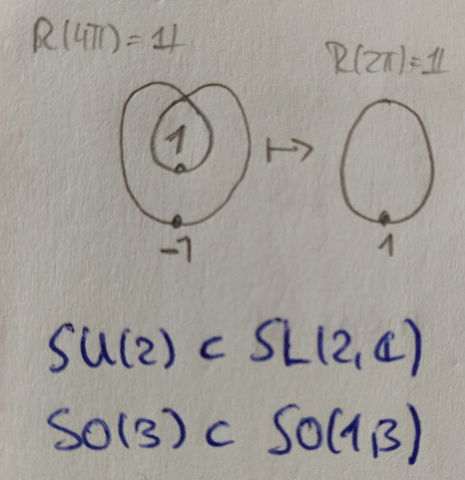
\includegraphics[width=0.7\linewidth]{gfx/doublecoverDiracSpinor}
	\caption{\itshape Double cover of the group, need to rotate by $4\pi$ to get back to the origin.}
	\label{fig:doublecoverdiracspinor}
\end{figure}

$\Rightarrow \psi_L, \psi_R$ transform under the irreducible representation of SO(1,3), $\psi=(\psi_L, \psi_R)^T$ only transforms under the reducible representation of Spin(1,3).

\subsection{Lorentz tensor- and spinor-fields}
Fields $\psi(x)$ transforming under Lorentz transformations of the coordinates $x^\mu \rightarrow x^{\prime \mu} = \Lambda^\mu_\nu x^\nu$ as
\begin{equation}
\label{eq:fieldsLorentztrafo}
	\psi(x) \rightarrow \psi^\prime(x^\prime) = D(\Lambda) \psi(\Lambda^{-1}x^\prime)
\end{equation}
with the \todo{Work through gregors script on Lorentz group}
Spinor representations of $L^\uparrow_+$ are ordinary representations of $SL(2, \mathbb{C})$, which is the double cover of $L^\uparrow_+ ≡ SO(3, 1)$.





